\chapter{Fourier Analysis}
\label{chapter:fourier_analysis}


\section{Introduction}

We need a more precise language to talk about the effect of
linear filters, and the different image components, than to say
``sharp'' and ``blurry'' parts of the image.    The Fourier transform
provides that precision. By analogy with temporal frequencies, which describe how quickly signals vary over time,
a {\bf spatial frequency} describes how quickly a signal varies over space.
The Fourier transform lets us describe a signal as a sum of complex
exponentials, each of a different spatial frequency.

Fourier transforms are the basis of a number of computer vision approaches and are an important tool to understand images and how linear spatially invariant filters transform images. There are also important to understand modern representations such as positional encoding popularized by transformers \cite{vaswani2017attention}. 

\section{Image Transforms}

Sometimes it is useful to transform the image pixels into another representation that might reveal image properties that can be useful for solving vision tasks. Before we saw that linear filtering is a useful way of transforming an image. Linear image transforms with the form $\mathbf{x} =  \mathbf{H} \boldimgin$ can be thought of as a way of changing the initial pixels representation of $\boldimgin$ into a different representation in $\mathbf{x}$. 
\marginnote{We use $\mathbf{x}$ to denote an intermediate representation. The representation might not be an image.}
This representation is specially interesting when it  can  be inverted so that the original pixels can be recovered as $\boldimgin =  \mathbf{H}^{-1} \mathbf{x}$. The Fourier transform is one of those representations. A useful representation $\mathbf{x}$ should have a number of interesting properties not immediately available in the original pixels of $\boldimgin$. 




\section{Fourier Series}

%Joseph Fourier, French mathematician, studied how heat propagated inside a body. The goal was to predict precisely the temperature at every point inside a body at a given instant. The propagation of heat is described by a partial differential equation for which, despite its simple form, no general solution existed at the time. 

%In 1822, Fourier showed that trigonometric functions were solutions for the heat equation and that they could be used as basis to obtain a general solution to the problem. His initial paper was rejected for publication by Lagrange \cite{}, but his ideas were published later in his famous book {\it Theorie de la chaleur} \cite{},  and have become one of the most important mathematical tools in science and engineering. 


In 1822, French mathematician and engineer Joseph Fourier, as part of his work on the study on heat propagation, showed that 
any periodic signal could be written as an infinite sum of trigonometric functions (cosine and sine functions).  His ideas were published in his famous book \booktitle{Theorie de la Chaleur} \cite{Fourier09}, and the {\bf Fourier series} has become one of the most important mathematical tools in science and engineering. 


%trigonometric functions were solutions for the heat equation and that they could be used as basis to obtain a general solution to the problem. His initial paper was rejected for publication by Lagrange \cite{}, but his ideas were published later in his famous book {\it Theorie de la chaleur} \cite{},  and have become one of the most important mathematical tools in science and engineering. 



Fourier showed that any function, $\img (t)$ defined in the interval $t \in (0,\pi)$, could be expressed as an infinite linear combination of harmonically related sinusoids,
\begin{equation}
\img (t) = a_1 \sin (t) + a_2 \sin (2t) + a_3 \sin (3t) + ...
\end{equation}
and that the value of the coefficients $a_n$ could be computed as the area of the curve $\img(t) \sin (nt)$. Precisely,
\begin{equation} 
a_n = \frac{2}{\pi} \int_0^\pi  \img (t) \sin (nt) dt
\end{equation}
 However, the sum is only guaranteed to converge to the function $\img (t)$ within the interval $t \in (0,\pi)$. In fact, the resulting sum, for any values $a_n$, is a {\bf periodic function} with period $2\pi$ and is anti-symmetric with respect to the origin, $t=0$. %The conditions under which this series converges to the function $f(t)$ were studied by Cauchy. 

One of Fourier's original examples of {\bf sine series} 
\index{Sine series}
is the expansion of the ramp signal $\img (t)=t/2$. This series was first introduced by Euler. Fourier showed that his theory explained why a ramp could be written as the following infinite sum:
\begin{equation}
\frac{1}{2} t =  \sin (t) - \frac{1}{2}  \sin (2t) + \frac{1}{3} \sin (3t) - \frac{1}{4}  \sin (4t) + ...
\end{equation}
The result of this series approximates the ramp with increasing accuracy as we add more terms. The plots in \fig{\ref{fig:FourierSeries6}} show each of the weighted sine functions (on top) and the resulting partial sum (bottom graphs). We can see how adding {\bf higher frequency} sines adds more details to the resulting function making it closer to the ramp. These plots show the signal in the interval $t \in (-4 \pi, 4 \pi)$ to reveal the periodic nature of the result of the sine series. 

\begin{figure}[t]
\centerline{
\includegraphics[width=1\linewidth]{figures/Image_processing_fourier/FourierSeries6.eps}
}
%\begin{figure}[htpb!]
 %   \centering
 %   \includegraphics[width=0.75\linewidth]{FourierSeries4.eps}
%    \label{fig:star_symbol_learning}
\caption{Reconstruction of a ramp with the first five sine functions.}
\label{fig:FourierSeries6}
\end{figure}


It is useful to think of the {\bf Fourier series} of a signal as a {\bf change of representation} as shown in \fig{\ref{fig:FourierSeries5_representation}}. Instead of representing the signal by the sequence of values specified by the original function $\img (t)$, the same function can be represented by the infinite sequence of coefficients $a_n$. The coefficients $a_n$ give us an alternative description of the function $\img(t)$ and the rest of this chapter will be devoted to understand what this {\bf transformation} has to offer.  

\begin{figure}[t]
\centerline{
%\begin{figure}[h!]
 %   \centering
    \includegraphics[width=.9\linewidth]{figures/Image_processing_fourier/FourierSeries5_representation.eps}
%    \label{fig:star_symbol_learning}
%\end{figure}
}
\caption{Two representations for the ramp 
function. (left) Time domain. (right) Fourier domain with coefficients of the sine series.%function: time domain (left), Fourier domain (right): coefficients of the sine series.
}
\label{fig:FourierSeries5_representation}
\end{figure}

Fourier series can also be written as sums of different sets of harmonic functions. For instance, using cosine functions we can describe the ramp function also as: 
\begin{equation}
\frac{1}{2} t =  \frac{\pi}{4}  - \frac{2}{\pi} \cos (t) - \frac{2}{3^2 \pi}  \cos (3t) - \frac{2}{5^2 \pi}  \cos (5t) - ...
\end{equation}
 The cosine and sine series of the same function are only equal in the interval $t \in (0, \pi)$, and result in different periodic extensions outside that interval.

The fields of signal and image processing have introduced different types of Fourier series. In the next sections we will study how these series are applied to describe discrete images using discrete sine and cosine functions and then we will focus on using complex exponentials. The representation using Fourier series is important for studying linear systems and convolutions. 

\section{Continuous and Discrete Waves}

Now that we have seen the importance of sine waves as a tool to represent signals, let's describe them in a bit more detail.  

%Let's start by defining a very important family of signals: the sine wave. 
%\begin{comment}

%In 1807, Fourier demonstrated that any periodic signal could be written as an infinite sum of cosine and sine functions.  

The {\bf continuous time sine wave} is
\begin{equation}
s\left(t\right) = A \sin\left(w ~t - \theta \right)
\end{equation}
where $A$ is the {\bf amplitude}, $w$ is the {\bf frequency}, and $\theta$ is the {\bf phase}. The wave signal is periodic with a period $T=2 \pi / w$. 

\marginnote{
\centerline{
\includegraphics[width=.4\linewidth]{figures/Image_processing_fourier/amplitudeandperiod.eps}
}
}

In discrete time, the {\bf discrete time sine wave} is as follows
\begin{equation}
s\left[n\right] = A \sin\left(w ~n  - \theta \right)
\end{equation}
Note that the discrete sine wave will not be periodic for any arbitrary value of $w$. A discrete signal $\img \left[n\right]$ is periodic, if there exists $T \in \mathbb{N}$ such that $\img \left[n\right] = \img \left[n+mT\right]$ for all $m \in \mathbb{Z}$. For the discrete sine (and cosine) wave to be periodic the frequency has to be $w = 2 \pi K / N$ for $K,N \in \mathbb{N}$. If $K/N$ is an irreducible fraction, then the period of the wave will be $T = N$ samples. Although $\theta$ can have any value, here we will consider only the values $\theta=0$ and $\theta = \pi/2$, which correspond to the sine and cosine waves, respectively. 


In general, to make explicit the periodicity of the wave we will use the form:
\begin{equation}
s_k\left[n\right] = \sin\left( \frac{2 \pi}{N} \, k \, n \right)
\end{equation}

The same applies for the cosine:
\begin{equation}
c_k\left[n\right] = \cos\left(\frac{2 \pi}{N} \,k\,n \right)
\end{equation}
This particular notation makes sense when considering the set of periodic signals with period $N$, or the set of signals with finite support signals of length $N$ with $n \in \left[0, N-1\right]$. In such a case, $k \in \left[1, N/2\right]$ denotes the frequency (i.e., the number of wave cycles that will occur within the region of support). Note that if $k=0$ then $s\left[n\right]$ = 0 and $c\left[n\right]=1$ for all $n$. One can also verify that $c_{N-k} = c_k$, and $s_{N-k} = -s_k$. Therefore, for frequencies $k>N/2$ we find the same set of waves as the ones in the interval $s \in \left[1, N/2\right]$. \Fig{\ref{fig:contsignal}} shows some examples. 

\begin{figure}[t]
\centerline{
%\begin{array}{cc}
\sublabel{a}{
%\text{(a)}
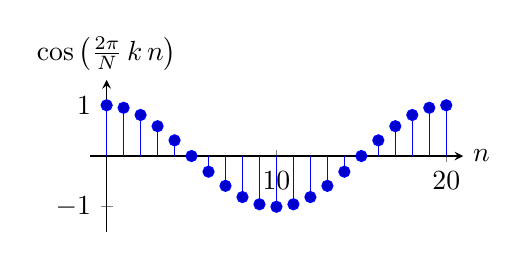
\begin{tikzpicture}
\begin{axis} [width=180pt,height=100pt,
	axis x line=middle, 
	axis y line=middle, 
	tick align=center,
	every axis x label/.style={at={(current axis.right of origin)},anchor=west},
	every axis y label/.style={at={(current axis.above origin)}, anchor=north east,above=0mm},
	xmin=-1, xmax=21,
	xtick={0,10,20},
	xlabel=$n$,
	ymin=-1.5, ymax=1.5,
	ytick={-1, 0,1},
	ylabel={$\cos\left(\frac{2 \pi}{N} \,k\,n \right)$},
	color=black]
 \addplot+[ycomb,domain=0:20,samples=21,samples y=0] 
 ({x}, {cos(deg(2*pi*x*1/20))}); 
\end{axis}
\end{tikzpicture}
}
%&
%\text{(b)}
\sublabel{b}{
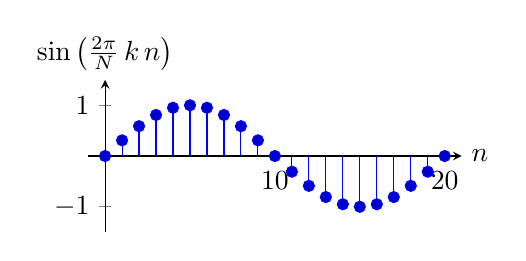
\begin{tikzpicture}
\begin{axis} [width=180pt,height=100pt,
	axis x line=middle, 
	axis y line=middle, 
	tick align=center,
	every axis x label/.style={at={(current axis.right of origin)},anchor=west},
	every axis y label/.style={at={(current axis.above origin)}, anchor=north east,above=0mm},
	xmin=-1, xmax=21,
	xtick={0,10,20},
	xlabel=$n$,
	ymin=-1.5, ymax=1.5,
	ytick={-1, 0,1},
	ylabel={$\sin\left(\frac{2 \pi}{N} \,k\,n \right)$}]
\addplot+[ycomb,domain=0:20,samples=21,samples y=0] 
 ({x}, {sin(deg(2*pi*x*1/20))}); 
\end{axis}
\end{tikzpicture}
}
%\end{array}
%\end{center}
}
\centerline{
%\[
%\begin{array}{cc}
\sublabel{c}{
%\text{(c)}
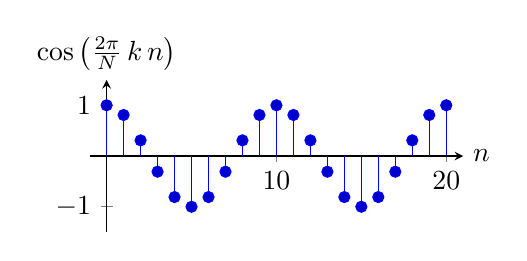
\begin{tikzpicture}
\begin{axis} [width=180pt,height=100pt,
	axis x line=middle, 
	axis y line=middle, 
	tick align=center,
	every axis x label/.style={at={(current axis.right of origin)},anchor=west},
	every axis y label/.style={at={(current axis.above origin)}, anchor=north east,above=0mm},
	xmin=-1, xmax=21,
	xtick={0,10,20},
	xlabel=$n$,
	ymin=-1.5, ymax=1.5,
	ytick={-1, 0,1},
	ylabel={$\cos\left(\frac{2 \pi}{N} \,k\,n \right)$},
	color=black]
 \addplot+[ycomb,domain=0:20,samples=21,samples y=0] 
 ({x}, {cos(deg(2*pi*x/10))}); 
\end{axis}
\end{tikzpicture}
}
%&
\sublabel{d}{
%\text{(d)}
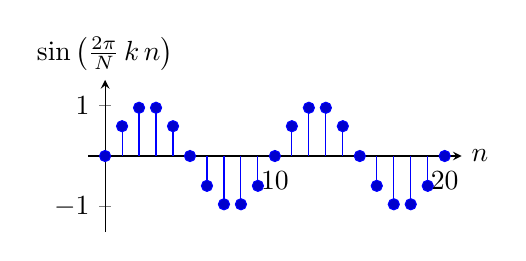
\begin{tikzpicture}
\begin{axis} [width=180pt,height=100pt,
	axis x line=middle, 
	axis y line=middle, 
	tick align=center,
	every axis x label/.style={at={(current axis.right of origin)},anchor=west},
	every axis y label/.style={at={(current axis.above origin)}, anchor=north east,above=0mm},
	xmin=-1, xmax=21,
	xtick={0,10,20},
	xlabel=$n$,
	ymin=-1.5, ymax=1.5,
	ytick={-1, 0,1},
	ylabel={$\sin\left(\frac{2 \pi}{N} \,k\,n \right)$}]
\addplot+[ycomb,domain=0:20,samples=21,samples y=0] 
 ({x}, {sin(deg(2*pi*x/10))}); 
\end{axis}
\end{tikzpicture}
}
%\end{array}
%\]
}
\centerline{
%\[
%\begin{array}{cc}
\sublabel{e}{
%\text{(e)}
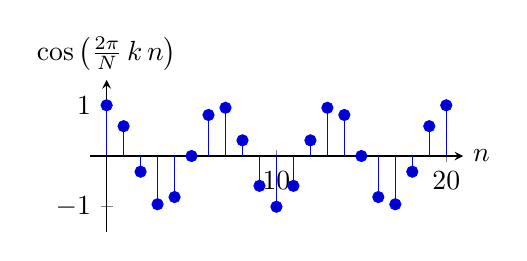
\begin{tikzpicture}
\begin{axis} [width=180pt,height=100pt,
	axis x line=middle, 
	axis y line=middle, 
	tick align=center,
	every axis x label/.style={at={(current axis.right of origin)},anchor=west},
	every axis y label/.style={at={(current axis.above origin)}, anchor=north east,above=0mm},
	xmin=-1, xmax=21,
	xtick={0,10,20},
	xlabel=$n$,
	ymin=-1.5, ymax=1.5,
	ytick={-1, 0,1},
	ylabel={$\cos\left(\frac{2 \pi}{N} \,k\,n \right)$},
	color=black]
 \addplot+[ycomb,domain=0:20,samples=21,samples y=0] 
 ({x}, {cos(deg(2*pi*x*3/20))}); 
\end{axis}
\end{tikzpicture}
}
%&
\sublabel{f}{
%\text{(f)}
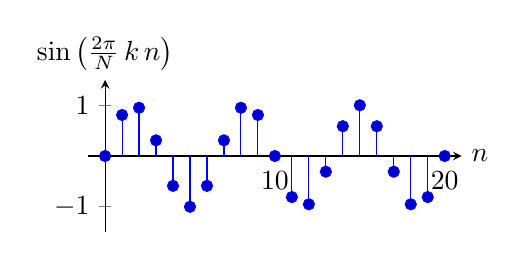
\begin{tikzpicture}
\begin{axis} [width=180pt,height=100pt,
	axis x line=middle, 
	axis y line=middle, 
	tick align=center,
	every axis x label/.style={at={(current axis.right of origin)},anchor=west},
	every axis y label/.style={at={(current axis.above origin)}, anchor=north east,above=0mm},
	xmin=-1, xmax=21,
	xtick={0,10,20},
	xlabel=$n$,
	ymin=-1.5, ymax=1.5,
	ytick={-1, 0,1},
	ylabel={$\sin\left(\frac{2 \pi}{N} \,k\,n \right)$}]
\addplot+[ycomb,domain=0:20,samples=21,samples y=0] 
 ({x}, {sin(deg(2*pi*x*3/20))}); 
\end{axis}
\end{tikzpicture}
}
%\end{array}
%\]
}
\caption{Sine and cosine waves with $A=1$ and $N=20$. Each row corresponds to $k=1$, $k=2$ and $k=3$. Note that for $k=3$ the waves oscillates three times in the interval $\left[0,N-1\right]$, but the samples in each oscillation are not identical, and it is only truly periodic once every $N$ samples. This is because $3/20$ is an irreducible fraction. }
\label{fig:contsignal}
\end{figure}

\begin{comment}

One remarkable property of sine and cosine waves is that the set of function $s_k$ and $c_k$ constitute what is called an orthogonal basis for all periodic discrete signals with period $N$, and also for all discrete signals of length $N$ (and a similar property exists also for continuous signals). Therefore, any such signal can be written as:
\begin{equation}
f\left[n\right] = a_0+ \sum_{k=1}^{N/2} a_k  \cos\left(\frac{2 \pi}{N} \,k\,n \right) + \sum_{k=1}^{N/2} b_k  \sin\left(\frac{2 \pi}{N} \,k\,n \right)
\end{equation}
were the coefficients $a_k$ and $b_k$ are constants. 
\begin{eqnarray}
\label{eq:fourier1}
a_0 &=& \frac{1}{N} \sum_{n=1}^{N-1}  \, f\left[n\right] \nonumber \\
a_k &=& \frac{2}{N} \sum_{n=1}^{N-1}   \, f\left[n\right] \cos\left(\frac{2 \pi}{N} \,k\,n \right) \nonumber \\
b_k &=& \frac{2}{N} \sum_{n=1}^{N-1}   \, f\left[n\right] \sin\left(\frac{2 \pi}{N} \,k\,n \right)
\end{eqnarray}
The set of coefficients ($a_k$, $b_k$) provide an alternative representation of the signal $f$ to the one provided by its sample values $f\left[n\right]$. As shown in equations \ref{eq:fourier1}, the coefficients ($a_k$, $b_k$) are a linear transformation of the samples $f\left[n\right]$.


The same analysis can be extended to 2 dimensions. In 2D, the discrete sine and cosine waves are:
\begin{equation}
s_{u,v}\left[n,m\right] = A \sin \left(2 \pi \left( \frac{u\,n}{N}  + \frac{v\,m}{M}  \right) \right)
\end{equation}
\begin{equation}
c_{u,v}\left[n,m\right] = A \cos \left(2 \pi \left( \frac{u\,n}{N}  + \frac{v\,m}{M}  \right) \right)
\end{equation}

\begin{figure}[h]
\begin{center}
\[
\begin{array}{ccc}
\text{a)}
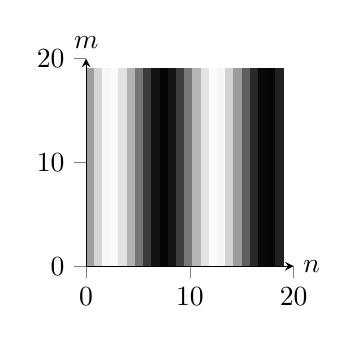
\begin{tikzpicture} 
\begin{axis}[width=120pt,height=120pt,
	mesh/ordering=y varies,
	view={0}{90},
	ymin=0, ymax=20,
	xmin=0, xmax=20,
	axis on top, 
	axis x line=bottom, 
	axis y line=left, 
	tick align=outside,
	every axis x label/.style={at={(current axis.right of origin)},anchor=west},
	every axis y label/.style={at={(current axis.north west)}, anchor=north west,above=0mm},
	xlabel={$n$}, ylabel={$m$}, zlabel={$z$}
	]  
\addplot3[surf,colormap/blackwhite,domain=0:19,shader=flat]  {sin(deg(2*pi*x*2/20 + 2*pi*y*0/20))};
\end{axis} 
\end{tikzpicture} 
&
\text{b)}
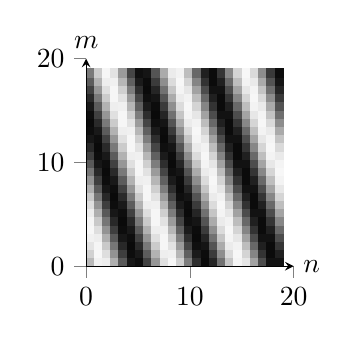
\begin{tikzpicture} 
\begin{axis}[width=120pt,height=120pt,
	mesh/ordering=y varies,
	view={0}{90},
	ymin=0, ymax=20,
	xmin=0, xmax=20,
	axis on top, 
	axis x line=bottom, 
	axis y line=left, 
	tick align=outside,
	every axis x label/.style={at={(current axis.right of origin)},anchor=west},
	every axis y label/.style={at={(current axis.north west)}, anchor=north west,above=0mm},
	xlabel={$n$}, ylabel={$m$}, zlabel={$z$}
	]  
\addplot3[surf,colormap/blackwhite,domain=0:19,shader=flat]  {sin(deg(2*pi*x*3/20 + 2*pi*y*1/20))};
\end{axis} 
\end{tikzpicture} 
&
\text{c)}
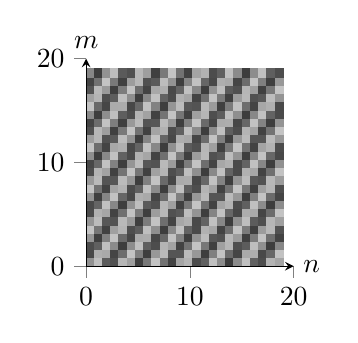
\begin{tikzpicture} 
\begin{axis}[width=120pt,height=120pt,
	mesh/ordering=y varies,
	view={0}{90},
	ymin=0, ymax=20,
	xmin=0, xmax=20,
	axis on top, 
	axis x line=bottom, 
	axis y line=left, 
	tick align=outside,
	every axis x label/.style={at={(current axis.right of origin)},anchor=west},
	every axis y label/.style={at={(current axis.north west)}, anchor=north west,above=0mm},
	xlabel={$n$}, ylabel={$m$}, zlabel={$z$}
	]  
\addplot3[surf,colormap/blackwhite,domain=0:19,shader=flat]  {sin(deg(2*pi*x*7/20 - 2*pi*y*5/20))};
\end{axis} 
\end{tikzpicture} 
\end{array}
\]
\end{center}
\caption{2D sine waves with $N=M=20$. The frequency values are: a) $u=2, v=0$, b) $u=3, v=1$, c) $u=7,v=-5$} 
\label{fig:disc2Dsignal}
\end{figure}


\end{comment}


\subsection{Sines and Cosines in 2D}

The same analysis can be extended to two dimensions (2D). In 2D, the discrete sine and cosine waves are as follows:

%Let's start by defining two very useful image families: the discrete sine and cosine waves. They are defined as:
 \begin{equation}
 s_{u,v}\left[n,m\right] = A \sin \left(2 \pi \left( \frac{u\,n}{N}  + \frac{v\,m}{M}  \right) \right)
 \end{equation}
 \begin{equation}
 c_{u,v}\left[n,m\right] = A \cos \left(2 \pi \left( \frac{u\,n}{N}  + \frac{v\,m}{M}  \right) \right)
 \end{equation}
 where $A$ is the amplitude and $u$ and $v$ are the two spatial frequencies and define how fast or slow the waves change along the spatial dimensions $n$ and $m$. \Fig{\ref{fig:disc2Dsignal}} shows some examples. 
 \begin{figure}[h]
 \centerline{
 %\[
 %$
 %\begin{array}{ccc}
 %\text{(a)}
\sublabel{a}{
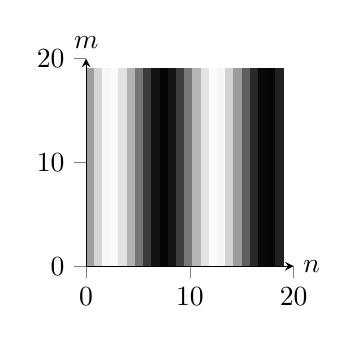
\begin{tikzpicture} 
 \begin{axis}[width=120pt,height=120pt,
 	mesh/ordering=y varies,
 	view={0}{90},
 	ymin=0, ymax=20,
 	xmin=0, xmax=20,
 	axis on top, 
 	axis x line=bottom, 
 	axis y line=left, 
 	tick align=outside,
 	every axis x label/.style={at={(current axis.right of origin)},anchor=west},
 	every axis y label/.style={at={(current axis.north west)}, anchor=north west,above=0mm},
 	xlabel={$n$}, ylabel={$m$}, zlabel={$z$}
 	]  
 \addplot3[surf,colormap/blackwhite,domain=0:19,shader=flat]  {sin(deg(2*pi*x*2/20 + 2*pi*y*0/20))};
 \end{axis} 
 \end{tikzpicture} 
 }
 %&
 %\text{(b)}
\sublabel{b}{
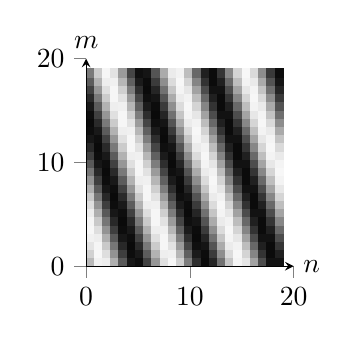
\begin{tikzpicture} 
 \begin{axis}[width=120pt,height=120pt,
 	mesh/ordering=y varies,
 	view={0}{90},
 	ymin=0, ymax=20,
 	xmin=0, xmax=20,
 	axis on top, 
 	axis x line=bottom, 
 	axis y line=left, 
 	tick align=outside,
 	every axis x label/.style={at={(current axis.right of origin)},anchor=west},
 	every axis y label/.style={at={(current axis.north west)}, anchor=north west,above=0mm},
 	xlabel={$n$}, ylabel={$m$}, zlabel={$z$}
 	]  
 \addplot3[surf,colormap/blackwhite,domain=0:19,shader=flat]  {sin(deg(2*pi*x*3/20 + 2*pi*y*1/20))};
 \end{axis} 
 \end{tikzpicture} 
 }
 %&
 %\text{(c)} 
\sublabel{c}{
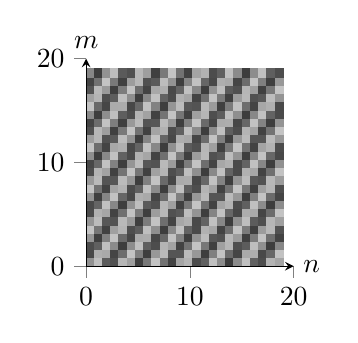
\begin{tikzpicture} 
 \begin{axis}[width=120pt,height=120pt,
 	mesh/ordering=y varies,
 	view={0}{90},
 	ymin=0, ymax=20,
 	xmin=0, xmax=20,
 	axis on top, 
 	axis x line=bottom, 
 	axis y line=left, 
 	tick align=outside,
 	every axis x label/.style={at={(current axis.right of origin)},anchor=west},
 	every axis y label/.style={at={(current axis.north west)}, anchor=north west,above=0mm},
 	xlabel={$n$}, ylabel={$m$}, zlabel={$z$}
 	]  
 \addplot3[surf,colormap/blackwhite,domain=0:19,shader=flat]  {sin(deg(2*pi*x*7/20 - 2*pi*y*5/20))};
 \end{axis} 
 \end{tikzpicture} 
 }
 %\end{array}
 %\]
 %$
 }
 \caption{2D sine waves with $N=M=20$. The frequency values are (a) $u=2, v=0$; (b) $u=3, v=1$; (c) $u=7,v=-5$.} 
 \label{fig:disc2Dsignal}
 \end{figure}

In 2D, the sine and cosine waves can also be described using polar coordinates for encoding the frequency: radial frequency, $\sqrt{u^2+v^2}$, and orientation, $\angle (u,v)$. 
\index{Radial frequency}
%In discrete time (setting $A=1$), we can write:
%\begin{equation}
%e_k\left[n\right] = \exp \left( j \frac{2 \pi}{N} \,k \,n \right) = \cos \left(\frac{2 \pi}{N} \,k \,n \right) + j \sin \left( \frac{2 \pi}{N} \,k \,n \right)
%\end{equation}







\subsection{Complex Exponentials}

Another important signal is the complex exponential wave: 
\begin{equation}
e_{u}\left[n\right] = \exp \left(2 \pi j   \frac{u\, n}{N}   \right) 
\end{equation}

Complex exponentials are related to cosine and sine waves by Euler's formula:
\index{Euler's formula}
\begin{equation}
\label{eq:euler}
\exp \left(j a\right) = \cos (a) + j \sin (a)
\end{equation}
\Fig{\ref{fig:complexexponential}} shows the one dimensional (1D) discrete complex exponential function (for $v=0$). As the values are complex, the plot shows in the $x$-axis the real component and in the $y$-axis the imaginary component. As $n$ goes from 0 to $N-1$ the function rotates along the complex circle of unit magnitude.


\begin{figure}[t]
\centerline{
%\[
%$
%\begin{array}{cc}
%\text{(a)}
\sublabel{a}{
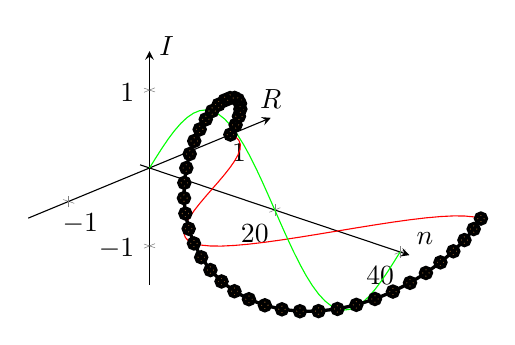
\begin{tikzpicture} 
\begin{axis}[view={42}{30}, width=230pt,
	axis x line=middle, 
	axis y line=middle, 
	axis z line=middle, 
	tick align=center,
	ymin=-1.5, ymax=1.5,
	zmin=-1.5, zmax=1.5,
	xmin=-1.5, xmax=41.5,
	%,anchor=near ticklabel
	%every axis z label/.style={at={(0,0,1)},left=0mm,above=0mm},
	%every axis x label/.style={at={(current axis.right of origin)},anchor=west,left=16mm,above=2mm},
	%every axis y label/.style={at={(current axis.above origin)},anchor=north east,above=-8mm,left=57mm},
        xlabel=$n$,ylabel=$\mathbb{R}$,zlabel=$\mathbb{I}$,
        %y dir=reverse,
        every axis y label/.append style={at=(ticklabel* cs:1.0),above=0mm},
        every axis x label/.append style={at=(ticklabel* cs:1.1)},
        every axis z label/.append style={at=(ticklabel* cs:1.1)}
]
 \addplot3[domain=0:40,samples=41,samples y=0,draw=red] 
 ({x}, {cos(deg(2*pi*1*x/40))}, {0}); 
\addplot3[domain=0:40,samples=41,samples y=0,draw=green] 
 ({x}, {0}, {sin(deg(2*pi*1*x/40))}); 
 \addplot3+[domain=0:40,samples=41,samples y=0,very thick,draw=black] 
 %({cos(deg(x))}, {x}, {sin(deg(x))}); 
 ({x}, {cos(deg(2*pi*1*x/40))}, {sin(deg(2*pi*1*x/40))}); 
 \end{axis} 
 \end{tikzpicture}
 }
 %&
%\text{(b)}
\sublabel{b}{
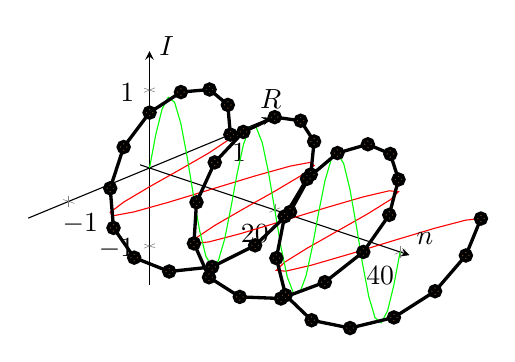
\begin{tikzpicture} 
\begin{axis}[view={42}{30}, width=230pt,
	axis x line=middle, 
	axis y line=middle, 
	axis z line=middle, 
	tick align=center,
	ymin=-1.5, ymax=1.5,
	zmin=-1.5, zmax=1.5,
	xmin=-1.5, xmax=41.5,
	%,anchor=near ticklabel
	%every axis z label/.style={at={(0,0,1)},left=0mm,above=0mm},
	%every axis x label/.style={at={(current axis.right of origin)},anchor=west,left=16mm,above=2mm},
	%every axis y label/.style={at={(current axis.above origin)},anchor=north east,above=-8mm,left=57mm},
        xlabel=$n$,ylabel=$\mathbb{R}$,zlabel=$\mathbb{I}$,
        %y dir=reverse,
        every axis y label/.append style={at=(ticklabel* cs:1.0),above=0mm},
        every axis x label/.append style={at=(ticklabel* cs:1.1)},
        every axis z label/.append style={at=(ticklabel* cs:1.1)}
]
 \addplot3[domain=0:40,samples=41,samples y=0,draw=red] 
 ({x}, {cos(deg(2*pi*3*x/40))}, {0}); 
\addplot3[domain=0:40,samples=41,samples y=0,draw=green] 
 ({x}, {0}, {sin(deg(2*pi*3*x/40))}); 
 \addplot3+[domain=0:40,samples=41,samples y=0,very thick,draw=black] 
 %({cos(deg(x))}, {x}, {sin(deg(x))}); 
 ({x}, {cos(deg(2*pi*3*x/40))}, {sin(deg(2*pi*3*x/40))}); 
 \end{axis} 
 \end{tikzpicture}
 }
%\end{array}
%\]
%$
}
%\vspace{-0.5in}
\caption{Complex exponential wave with (a) $N=40$, $k=1$, $A=1$; and (b) $N=40$, $k=3$, $A=1$. The red and green curves show the real and imaginary waves. The black line is the complex exponential. The dots correspond to the discrete samples.} 
\label{fig:complexexponential}
\end{figure}


In 2D, the complex exponential wave is
\begin{equation}
e_{u,v}\left[n,m\right] = \exp \left(2 \pi j \left(  \frac{u\, n}{N}  + \frac{v\,m}{M}  \right) \right) 
\end{equation}
where $u$ and $v$ are the two spatial frequencies. Note that complex exponentials in 2D are separable. This means they can be written as the product of two 1D signals:
\begin{equation}
e_{u,v}\left[n,m\right]   = e_{u}\left[n\right] e_{v}\left[m\right] 
\end{equation}

 

%
%The set of functions $e_k\left[n\right]$, with $k\in\left[0,N-1\right]$, form an orthogonal basis for discrete signals of length $N$. In fact, 
%\begin{equation}
%\left<e_k, e_r \right> = \sum_{n=0}^{N-1} e_k\left[n\right] e^*_r\left[n\right] = N \delta \left[k-r\right] = 
% \begin{cases}
%    N       & \quad \text{if } k=r\\
%    0       & \quad \text{if } k \neq r\\
%  \end{cases}
%\end{equation}

A remarkable property is that the complex exponentials form an orthogonal basis for discrete signals and images of finite length. For images of size $N \times M$,
\begin{equation}
\left<e_{u,v}, e_{u',v'} \right> = \sum_{n=0}^{N-1} \sum_{m=0}^{M-1} e_{u,v}\left[n,m\right] e^*_{u',v'}\left[n,m\right] = MN \delta \left[u-u'\right]\delta \left[v-v'\right] 
\end{equation}
Therefore, any finite length discrete image can be decomposed as a linear combination of complex exponentials. 


%\begin{eqnarray}
%\label{eq:euler}
%\cos{ \left( 2\pi \left( \frac{u\, n}{N} + \frac{v m}{M} \right) \right) } &=& \frac{1}{2} \left( e_{u,v}\left[n,m\right]  +  e^*_{u,v}\left[n,m\right]  \right) \\
%\sin{ \left( 2\pi \left( \frac{u\, n}{N} + \frac{v m}{M} \right) \right) } &=& \frac{-j}{2} \left( e_{u,v}\left[n,m\right]  - e^*_{u,v}\left[n,m\right]  \right)
%\end{eqnarray}
%
%


\section{The Discrete Fourier Transform}

In this chapter we will focus on the discrete Fourier transform as it provides important tools to understand the behavior of signals and systems (e.g., sampling and convolutions). For a more detailed study of other transforms and the foundations of Fourier series we refer the reader to other specialized books in signal and image processing .

\subsection{Discrete Fourier Transform and Inverse Transform}

The {\bf Discrete Fourier Transform} (DFT) transforms an image $\img \left[n,m \right]$, of finite size $N \times M$, into the complex image Fourier transform $\capitalimg \left[u,v \right]$ as:
\begin{equation}
\capitalimg \left[u,v \right] =  
\mathcal{F} \left\{ \img \left[n,m \right] \right\}
=
\sum_{n=0}^{N-1} \sum_{m=0}^{M-1} \, \img \left[n,m \right] 
\exp{ \left( -2\pi j \left( \frac{u\, n}{N} + \frac{v\, m}{M} \right) \right)}
\label{eq:fourier}
\end{equation}
We will call $\capitalimg \left[u,v \right]$ the Fourier transform of $\img \left[m,n \right]$. We will often represent the relationship between the signal as its transform as:
\begin{equation}
\img \left[n,m \right] \xrightarrow{\mathscr{F}} \capitalimg \left[u,v \right]
\end{equation}


By applying 
$\frac{1}{MN} \sum_{u=0}^{M-1} \sum_{v=0}^{N-1}$
to both sides of \eqn{\ref{eq:fourier}} and exploiting the orthogonality between distinct Fourier basis elements, we find the {\bf inverse Fourier transform} relation
\begin{equation}
\img \left[n,m \right] = 
\mathcal{F}^{-1} \left\{ \capitalimg \left[u,v \right] \right\}
=
\frac{1}{NM} \sum_{u=0}^{N-1} \sum_{v=0}^{M-1} \capitalimg \left[u,v \right] 
\exp{ \left(+2\pi j \left(\frac{u\, n}{N} + \frac{v\, m}{M} \right) \right) }
\label{eq:inversefourier}
\end{equation}


As we can see from the inverse transform equation, we rewrite the image, instead of as a sum of offset pixel
values, as a sum of complex exponentials, each at a different frequency, called a spatial frequency for images because they describe
how quickly things vary across space.  From the inverse transform formula, we see that to construct an image
from a Fourier transform, $\capitalimg \left[u,v \right]$, we just add in the corresponding
amount of that particular complex exponential (conjugated).

As $\capitalimg \left[u,v \right]$ is obtained as a sum of complex exponential with a common period of $N,M$ samples, the function  $\capitalimg \left[u,v \right]$  is also periodic: $\capitalimg \left[u+aN,v+bM \right] = \capitalimg \left[u,v \right]$ for any $a,b \in \mathbb{Z}$.
Also the result of the inverse DFT is a periodic image. Indeed you can verify from \eqn{\ref{eq:inversefourier}} that $\img \left[n+aN,m+bM \right] = \img \left[n,m \right]$ for any $a,b \in \mathbb{Z}$. 


% Source: https://en.wikipedia.org/wiki/Cooley%E2%80%93Tukey_FFT_algorithm

Using the fact that $e_{N-u, M-v} = e_{-u,-v}$, another equivalent way to write for the Fourier transform is to sum over the frequency interval $\left[-N/2, N/2\right]$ and $\left[-M/2, M/2\right]$. This is especially useful for the inverse that can be written as:
\begin{equation}
\img \left[n,m \right] = \frac{1}{NM} \sum_{u=-N/2}^{N/2} \sum_{v=-M/2}^{M/2} \capitalimg \left[u,v \right] 
\exp{ \left(+2\pi j \left(\frac{u\, n}{N} + \frac{v\, m}{M} \right) \right) }
\label{eq:inversefourier2}
\end{equation}

This formulation allows us to arrange the coefficients in the complex plane so that the zero frequency, or DC, coefficient is at the center.  Slow, large variations correspond to complex exponentials of
frequencies near the origin.   If the amplitudes of the complex conjugate exponentials are the same, then their sum will represent a cosine wave;  if their amplitudes are opposite, it will be a sine
wave.  Frequencies further away from the origin represent faster
variation with movement across space. The DFT and its inverse in 1D are defined in the same way as shown in table \ref{table:tableFamilyFT}. 


One very important property is that the decomposition of a signal into a sum of complex exponentials is unique: there is a unique linear combination of the exponentials that will result in a given signal. 

\marginnote{The DFT became very popular thanks to the {\bf Fast Fourier Transform} (FFT) algorithm. The most common FFT algorithm is the Cooley–Tukey algorithm \cite{Cooley1965} that reduces the computation cost from $O(N^2)$ to $O(N \log N)$.}[-1.1in]
\index{Fast Fourier transform}

\subsection{Matrix Form of the Fourier Transform}



As the DFT is a linear transform we can also write the DFT in matrix form, with one basis per row. In 1D, the matrix for the DFT is as follows:

\begin{equation}
    \mathbf{F} = \begin{bmatrix}
1 & 1 & 1 & \dots & 1\\ %u=0
1 & \exp{ \left(-2\pi j \frac{1}{N} \right)} & \exp{ \left(-2\pi j \frac{2}{N} \right)} & \dots & \exp{ \left(-2\pi j \frac{N-1}{N} \right)}\\ %u=1
1 & \exp{ \left(-2\pi j \frac{2}{N} \right)} & \exp{ \left(-2\pi j \frac{4}{N} \right)} & \dots & \exp{ \left(-2\pi j \frac{2\, (N-1)}{N} \right)}\\ %u=2
\vdots & \vdots & \vdots & ~ & \vdots \\
1 & \exp{ \left(-2\pi j \frac{(N-1)}{N} \right)} & \exp{ \left(-2\pi j \frac{(N-1)\, 2}{N} \right)} & \dots & \exp{ \left(-2\pi j \frac{(N-1)\, (N-1)}{N} \right)}\
\end{bmatrix}
\end{equation}
Each entry in the matrix is $\mathbf{F}_{u,n} = \exp{ \left(-2\pi j \frac{u\, n}{N} \right)}$, with $u$ indexing rows and $n$ indexing columns. Note that $\mathbf{F}$ is a symmetric matrix. The inverse of the DFT is the complex conjugate: $\mathbf{F}^{-1} = \mathbf{F}^{*}$.

Working in 1D, as we did before, allows us to visualize the transformation matrix. \Fig{\ref{fig:colorDFT}} shows a color visualization of the
complex-value matrix for the 1D DFT, which when used as a multiplicand yields the Fourier transform of 1D vectors.  Many Fourier transform properties and symmetries can be observed from inspecting that matrix. %Note that this matrix also has some similarities with the matrix used to compute the 1D DCT.


\begin{figure}[t]
\centerline{
\includegraphics[width=0.7\linewidth]{figures/Image_processing_fourier/visualization_DFT_color.eps}}
\caption{Visualization of the discrete Fourier transform as a matrix.  The signal to be
 transformed forms the entries of the column vector at right.  The
 complex values of the Fourier transform matrix are indicated by the color,
 with the key in the bottom left.  In the vector at the right, black
 values indicate zero.
} 
\label{fig:colorDFT}
\end{figure}

\subsection{Visualizing the Fourier Transform}


When computing the DFT of a real image, we will not be able to write the analytic form of the result, but there are a number of properties that will help us to interpret the result. \Fig{\ref{fig:DFT_a}} shows the Fourier transform of a $64 \times 64$ resolution image of a cube.
As the DFT results in a complex representation, there are two possible ways of writing the result. Using the real and imaginary components:
\begin{equation}
\capitalimg \left[u,v \right] = Re \left\{\capitalimg \left[u,v \right] \right\}  + j \, Imag \left\{\capitalimg \left[u,v \right] \right\}
\end{equation}
where $Re$ and $Imag$ denote the real and imaginary part of each Fourier coefficient. Or using a polar decomposition:
\begin{equation}
\capitalimg \left[u,v \right]  = A \left[u,v \right] \, \exp{\left( j \, \theta\left[u,v \right]  \right)}
\end{equation}
where $A \left[u,v \right] \in \mathbb{R}^+$ is the amplitude and $\theta \left[u,v \right] \in \left[-\pi, \pi \right]$ is the phase. 
\Fig{\ref{fig:DFT_a}} shows both decompositions of the Fourier transform.


\begin{figure}[t]
\centerline{
\includegraphics[width=1\linewidth]{figures/Image_processing_fourier/dft_a.eps}
}
\caption{DFT of an image and visualization of (top) the real and imaginary components,
and (bottom) the amplitude and phase  of the Fourier transform.} 
\label{fig:DFT_a}
\end{figure}

Upon first learning about Fourier transforms, it may be a surprise for readers to learn that one can synthesize any image as a sum of complex exponentials (i.e., sines and cosines).  To help gain insight into how that works, it is informative to show examples of partial sums of complex exponentials. \Fig{\ref{fig:DFT_b}} shows partial sums of the Fourier components
of an image.  In each partial sum of $N$ components, we use the largest N components of the Fourier transform.
Using the fact that the Fourier basis functions are orthonormal, it is straightforward to show that this is the best least-squares reconstruction possible from each given number of Fourier basis
components.  This first image shows what is reconstructed from the largest Fourier component which turns out to be $\capitalimg \left[0,0 \right]$. This component encodes the DC value of the image, therefore the resulting image is just a constant. The next two components correspond to two complex conjugates of a very slow varying wave. And so on. As more components get added, the figure slowly emerges. In this example, the first 127 coefficients are sufficient for recognizing this 64$\times$64 resolution image.


\begin{figure}[t]
\centerline{
\includegraphics[width=1\linewidth]{figures/Image_processing_fourier/dft_b.eps}
}
\caption{Reconstructing an image from the $N$ Fourier coefficients of
  the largest amplitude.  The right frame shows the location, in the
  Fourier domain, of the $N$ Fourier coefficients, which when
  inverted, give the image at the left.
} 
\label{fig:DFT_b}
\end{figure}

\section{Useful Transforms}

It's useful to become adept at computing and manipulating
simple Fourier transforms.  For some simple cases, we can compute the analytic form of the Fourier transform.

\subsection{Delta Distribution}

The Fourier transform of the delta function $\delta \left[n,m \right]$ is
\begin{equation}
\mathcal{F} \left\{ \delta \left[n,m \right] \right\} = 
%X \left[u,v \right] =  
\sum_{n=0}^{N-1} \sum_{m=0}^{M-1} \, \delta \left[n,m \right] 
\exp{ \left( -2\pi j \left( \frac{u\, n}{N} + \frac{v\, m}{M} \right) \right)} = 1
\end{equation}
where the Fourier transform of the delta signal is 1. 
\begin{equation}
\delta \left[n,m \right] \xrightarrow{\mathscr{F}} 1
\end{equation}
If we think in terms of the inverse Fourier transform, this means that if we sum all the complex exponentials with a coefficient of 1, then all the values will cancel but the one at the origin, which results in a delta function:
\begin{equation}
\delta \left[n,m \right] = \frac{1}{NM} \sum_{u=-N/2}^{N/2} \sum_{v=-M/2}^{M/2}  
\exp{ \left(2\pi j \left(\frac{u\, n}{N} + \frac{v\, m}{M} \right) \right) }
\end{equation}

\subsection{Cosine and Sine Waves}

The Fourier transform of the cosine wave, $\cos{ \left( 2\pi \left( \frac{u_0\, n}{N} + \frac{v_0\, m}{M} \right) \right) }$, is:
\begin{eqnarray}
\sum_{n=0}^{N-1} \sum_{m=0}^{M-1} \, \cos{ \left( 2\pi \left( \frac{u_0 \, n}{N} + \frac{v_0 \, m}{M} \right) \right) }
\exp{ \left( -2\pi j \left( \frac{u\, n}{N} + \frac{v\, m}{M} \right) \right)} = \\ 
=\frac{1}{2} \left( \delta \left[u-u_0, v-v_0 \right] +  \delta \left[u+u_0, v+v_0 \right] \right)
\end{eqnarray}
This can be easily proven using Euler's \eqn{\ref{eq:euler}} and the orthogonality between complex exponentials. This results in the Fourier transform relationship: 
\begin{equation}
\cos{ \left( 2\pi \left( \frac{u_0\, n}{N} + \frac{v_0\, m}{M} \right) \right) } 
\xrightarrow{\mathscr{F}} 
\frac{1}{2} \left( \delta \left[u-u_0, v-v_0 \right] +  \delta \left[u+u_0, v+v_0 \right] \right)
\end{equation}

And for the sine wave, $\sin{ \left( 2\pi \left( \frac{u_0\, n}{N} + \frac{v_0 m}{M} \right) \right) }$, we have a  similar relationship:


\begin{equation}
\sin{ \left( 2\pi \left( \frac{u_0\, n}{N} + \frac{v_0 m}{M} \right) \right) } 
\xrightarrow{\mathscr{F}} 
\frac{1}{2j} \left( \delta \left[u-u_0, v-v_0 \right] - \delta \left[u+u_0, v+v_0 \right]\right)
\end{equation}

\Fig{\ref{fig:2ddftexampleswaves}} shows the DFT of several waves with different frequencies and orientations. 


\begin{figure}[t]
\centerline{
\includegraphics[width=1\linewidth]{figures/Image_processing_fourier/DFT_examples_waves.eps}
}
\caption{Some 2D Fourier transform pairs. Images are $64 \times 64$ pixels. The waves are cosine with frequencies $(1,2)$, $(5,0)$, $(10,7)$, $(11,-15)$. The last two examples show the sum of two waves and the product.  
} 
\label{fig:2ddftexampleswaves}
\end{figure}


\Fig{\ref{fig:2ddftexamples}} shows the 2D Fourier transforms of
some periodic signals.  The depicted signals all happen to be symmetric
about the spatial origin.  From the Fourier transform equation, one
can show that real and even input signals transform to real and even
outputs.  So for the examples of \fig{\ref{fig:2ddftexamples}}, we only
show the magnitude of the Fourier transform, which in this case is the
absolute value of the real component of the transform, and the
imaginary component happens to be zero for the signals we'll examine. Also, all these images but the last one are separable (they can be written as the product of two 1D signals). Therefore, their DFT is also the product of 1D DFTs.


\begin{figure}
\centerline{
\includegraphics[width=1\linewidth]{figures/Image_processing_fourier/DFT_toy_examples.eps}
}
\caption{Some two-dimensional Fourier transform pairs.
  Note the trends visible in the collection of transform pairs:  As
  the support of the image in one domain gets larger, the magnitude in
  the other domain becomes more localized.  A line transforms to a
  line oriented perpendicularly to the first. Images are $64 \times 64$ pixels, origin is in the center.
} 
\label{fig:2ddftexamples}
\end{figure}

\subsection{Box Function}
\label{sec:box_function}
The box function is a very useful function that we will use several times in this book. It is good to be familiar with its Fourier transform and how to compute it. The box function is defined as follows:
\begin{equation}
\text{box}_{L} \left[n \right] = 
\begin{cases}
    1       & \quad \text{if } -L \leq n \leq L  \\
    0       & \quad \text{otherwise.} 
  \end{cases}
\end{equation}

The box function takes values of 1 inside the interval $\left[ -L,L \right]$ and it is 0 outside. The duration of the box is $2L+1$.

It is useful to think of the box function as a finite length signal of length $N$ and to visualize its periodic extension outside of that interval. The following plot shows the box function for $L=5$ and $N=32$. In this plot, the box signal is defined between $-N/2=-16$ and $N/2-1=15$ and the rest is its periodic extension. 

\begin{figure}[h]
\centerline{
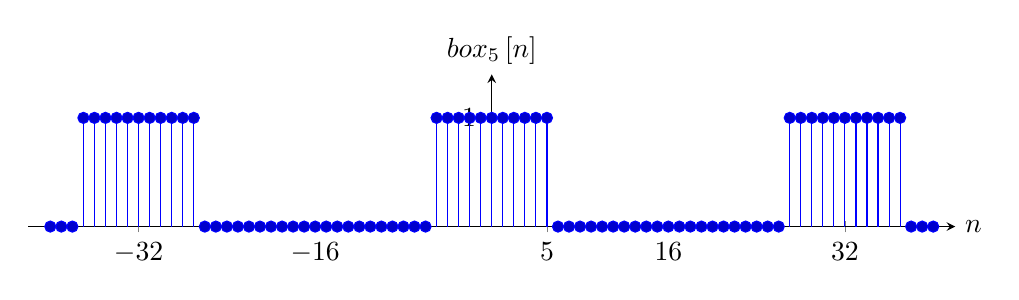
\begin{tikzpicture}
\begin{axis} [width=380,height=100pt,
	axis x line=bottom, 
	axis y line=middle, 
	tick align=center,
	every axis x label/.style={at={(current axis.right of origin)},anchor=west},
	every axis y label/.style={at={(current axis.above origin)}, anchor=north east,above=0mm},
	xmin=-42, xmax=42,
	xtick={-32,-16, -5 0, 5, 16,32},
	xlabel=$n$,
	ymin=0, ymax=1.4,
	ytick={0,...,1},
	ylabel={$\text{box}_{5} \left[n \right]$}]
 \addplot+[ycomb,domain=-40:40,samples=81,samples y=0] 
 ({x}, {(abs(mod(x,32))<6)+(abs(mod(x,32))>26)}); 
 \end{axis} 
\end{tikzpicture}
}
\caption{Box function for $L=5$ and $N=32$.}
\end{figure}

We will compute here the DFT of the finite length box function, with a length $N$. To compute the DFT we use the DFT definition and change the interval of the sum making use of the periodic nature of the terms inside the sum:
\begin{eqnarray}
\mathcal{F} \left\{ \text{box}_{L} \left[n \right] \right\} &=& 
\sum_{n=0}^{N-1} \, \text{box}_{L} \left[n \right] 
\exp{ \left( -2\pi j \frac{u\, n}{N} \right)} \\
&=& \sum_{n=-L}^{L} \,
\exp{ \left( -2\pi j \frac{u\, n}{N} \right)} 
\label{eq:boxdftderivation}
\end{eqnarray}

We can use the equation of the sum of a geometric series:
\begin{equation}
\sum_{n=-L}^{L} a^n = a^{-L} \sum_{n=0}^{2L} a^n = a^{-L} \frac{1-a^{2L+1}}{1-a} = \frac{a^{-(2L+1)/2}-a^{(2L+1)/2}}{a^{-1/2}-a^{1/2}}
\end{equation}
where $a$ is a constant. With $a = \exp{ \left( -2\pi j \frac{u}{N} \right)}$ we can write the sum in \eqn{\ref{eq:boxdftderivation}} as

\begin{eqnarray}
\sum_{n=-L}^{L} \,
\exp{ \left( -2\pi j \frac{u\, n}{N} \right)} & = & 
\frac{\exp{ \left( \pi j \frac{u(2L+1)}{N} \right)} - \exp{ \left( -\pi j \frac{u(2L+1)}{N} \right)}}
{\exp{ \left( \pi j \frac{u}{N} \right)} - \exp{ \left( - \pi j \frac{u}{N} \right)} } \\
& = & \frac{\sin \left( \pi u(2L+1)/N \right)}{\sin \left( \pi u/N \right)}
\label{eq:discrete_sinc_function}
\end{eqnarray}

This last function in \eqn{\ref{eq:discrete_sinc_function}} gets the special name of {\bf discrete sinc} function. 
\marginnote{
The discrete sinc function ({\bf sincd}) is defined as follows:
\begin{equation*}
\text{sincd}(x;a) = \frac{\sin(\pi x)}{a \sin (\pi x/a)}
\end{equation*}
Where $a$ is a constant. This is a symmetrical periodic function with a maximum value of 1.
}[-.6in]

In summary, we get that The DFT of the box function is the discrete sinc function: 
\begin{equation}
\text{box}_{L} \left[n \right] 
\xrightarrow{\mathscr{F}} 
\frac{\sin \pi u (2L+1)/N}{\sin \pi u/N} 
\end{equation}
We will denote the DFT of the box function, $\text{box}_{L} \left[n \right]$, capitalizing the first letter, $\text{Box}_{L} \left[u \right]$.
This function has its maximum value at $u=0$. The DFT, $\text{Box}_{L} \left[u \right]$, is a symmetric real function.
The following plot (\fig{\ref{fig:boxfilterdft}}) shows the DFT of the box with $L=5$, and $N=32$. One period of the DFT is contained in the interval $\left[ -16, 15 \right]$ and the rest is a periodic extension.

\begin{figure}[h]
\centerline{
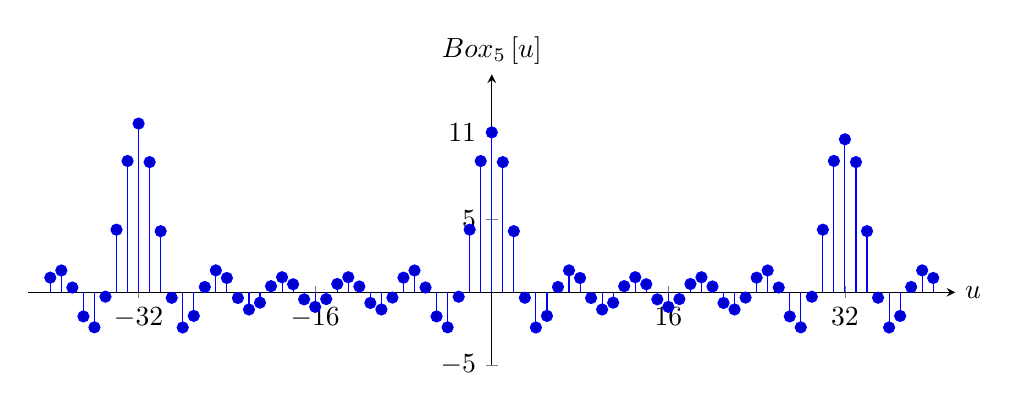
\begin{tikzpicture}
\begin{axis} [width=380pt,height=150pt,
	axis x line=middle, 
	axis y line=middle, 
	tick align=center,
	every axis x label/.style={at={(current axis.right of origin)},anchor=west},
	every axis y label/.style={at={(current axis.above origin)}, anchor=north east,above=0mm},
	xmin=-42, xmax=42,
	xtick={-32, -16, 0, 16, 32},
	xlabel=$u$,
	ymin=-5, ymax=15,
	ytick={-5,0,5,11},
	ylabel={$\text{Box}_{5} \left[u \right]$},
	color=black]
 \addplot+[ycomb,domain=-40:40,samples=81,samples y=0] 
 ({x}, {sin(deg(pi*(x+0.01)*(11)/32))) / sin(deg(pi*(x+0.01)/32)))}); 
\end{axis}
\end{tikzpicture}
}
\caption{DFT of the box filter with $L=5$, and $N=32$}
\label{fig:boxfilterdft}
\end{figure}

Now that we know how to compute the DFT of the 1D box, we can easily extend it to the 2D case. A 2D box is a separable function and can be written as the product of two box functions,
$\text{box}_{L_n, L_m} \left[n,m\right] = \text{box}_{L_n} \left[n\right] \text{box}_{L_m}\left[m\right]$. The DFT is the product of the two DFTs, 
\begin{equation}
\text{Box}_{L_n, L_m} \left[ u,v \right] = \text{Box}_{L_n} \left[ u\right] \text{Box}_{L_m} \left[ v\right].
\end{equation}

\Fig{\ref{fig:2ddftexamples}} shows several DFTs of 2D boxes of different sizes and aspect ratios.

\section{Discrete Fourier Transform Properties}
\label{section:DFTproperties}

It is important to be familiar with the properties for the DFT. Table \ref{table:tableDFT} summarizes some important transforms and properties. 


%For now, when we talk about images or signals we will assume they are periodic signals with periods $N$ and $M$ in each dimension. 


\begin{table}[t]
%\marginnote{{\bf Table \ref{table:tableDFT}}: Table of basic DFT transforms and properties.} % Hack to get the caption of the table in the margin.
%\faketablecaption{} % this updates the counter without plotting a caption.
\caption{Table of basic DFT transforms and properties.} % Hack to get the caption of the table in the margin.
%\caption{Table of basic DFT transforms and properties}
\begin{center}
\begin{tabular}{| c | c |}
\hline
\bf $\img \left[ n \right]$ & \bf $\capitalimg \left[u \right]$ \\
\hline \hline
$\img_1 \left[ n \right] \circ \img_2 \left[ n \right]$& $\capitalimg_1 \left[u \right] \capitalimg_2 \left[u \right]$ \\
\hline
$\img_1 \left[ n \right]$ $\img_2 \left[ n \right]$& $\frac{1}{N} \capitalimg_1 \left[u \right] \circ \capitalimg_2 \left[u \right]$ \\
\hline
$\img \left[ n-n_0 \right]$ & $\capitalimg \left[u \right] \exp{ \left( - 2 \pi j \frac{u n_0}{N} \right) }$  \\
\hline
$\delta \left[ n \right]$ & $1$ \\
\hline
$\exp{ \left( 2 \pi u_0 \frac{n}{N} \right) }$ &
$\delta \left[u-u_0 \right]$ \\
\hline
$\cos{ \left( 2 \pi u_0 \frac{n}{N} \right) }$ &
$\frac{1}{2} \left( \delta \left[u-u_0 \right] +  \delta \left[u+u_0\right] \right)$ \\
\hline
$\sin{ \left( 2 \pi u_0 \frac{n}{N} \right) }$ &
$\frac{1}{2j} \left( \delta \left[u-u_0 \right] -  \delta \left[u+u_0\right] \right)$ \\
\hline
$\text{box}_{L} \left[n \right]$ & $\frac{\sin \pi u (2L+1)/N}{\sin \pi u/N}$ \\
\hline
\end{tabular}
\end{center}
\label{table:tableDFT}
\end{table}

\subsection{Linearity}

The Fourier transform and its inverse are linear transformations:
%\begin{equation}
%DFT \left\{\alpha f\left[n,m \right] + \beta g\left[n,m \right] \right\} = \alpha F\left[u,v \right] +\beta G\left[u,v \right] 
%\end{equation}
\begin{equation}
\alpha \img_1 \left[n,m \right] + \beta \img_2 \left[ n,m \right]  
\xrightarrow{\mathscr{F}} 
\alpha \capitalimg_1 \left[u,v \right] + \beta \capitalimg_2 \left[ u,v \right]
\end{equation}
where $\alpha$ and $\beta$ are complex numbers. This property can be easily proven from the definition of the DFT. \Fig{\ref{fig:colorDFT}} shows a color visualization of the complex-value matrix for the 1D DFT.

\subsection{Separability}

An image is separable if it can be written as the product of two 1D signals, $\img \left[n,m \right] = \img_1\left[n \right] \img_2\left[m \right]$. If an image is separable, then its Fourier transform is separable:
%\begin{equation}
%DFT \left\{ f\left[n,m \right] \right\} = DFT \left\{ f_1\left[n \right] \right\} DFT \left\{ f_2\left[m \right] \right\}
%\end{equation}
%
%\begin{equation}
$\capitalimg \left[u,v \right] = \capitalimg_1 \left[u \right] \capitalimg_2 \left[v \right]$
%\end{equation}

\marginnote{{\bf Separability}. Although almost all images are not separable, some can be approximated by a separable image. Here is one example.
We can use the SVD decomposition to find a separable approximation to the image on the left. The result is shown on the right. 
\\[6pt]
\centerline{
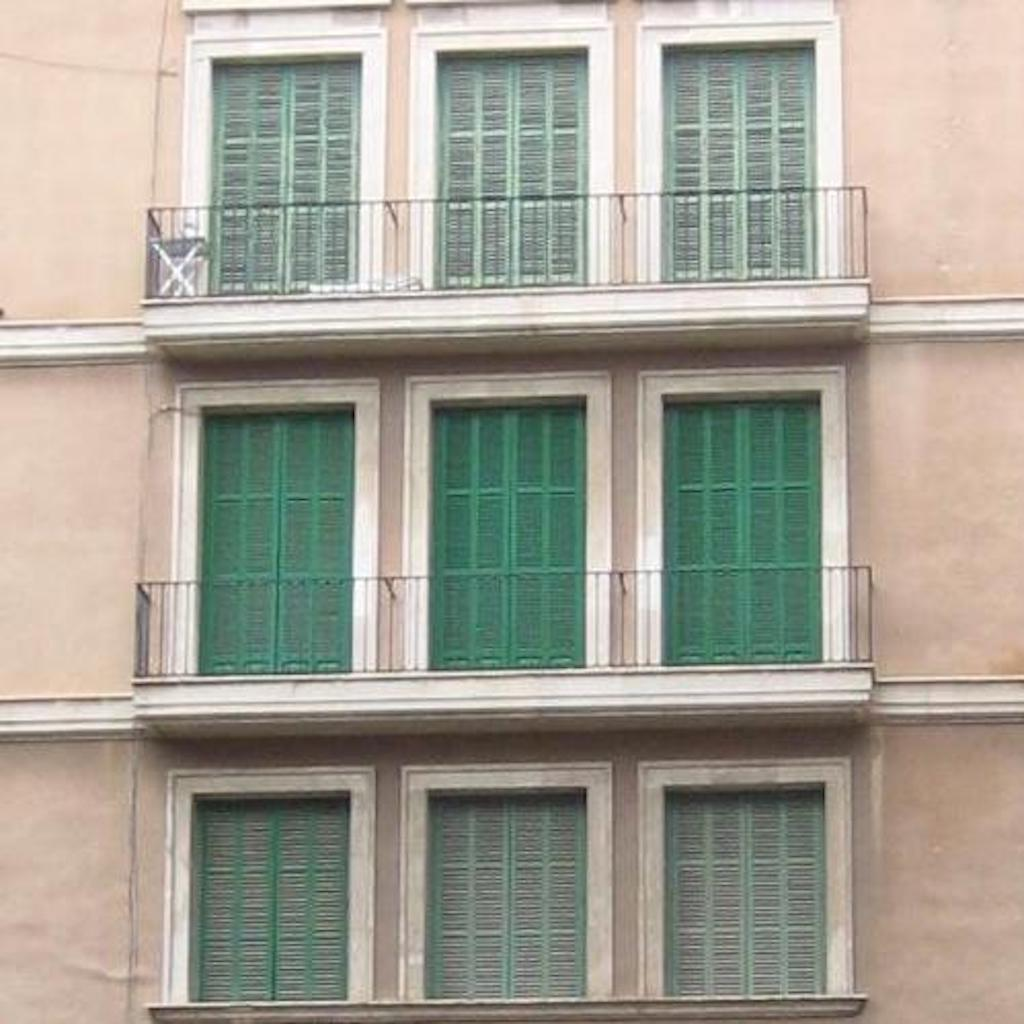
\includegraphics[width=.4\linewidth]{figures/Image_processing_fourier/facade1.jpg}
~~~~~~~~

\includegraphics[width=.4\linewidth]{figures/Image_processing_fourier/facade1aprox.jpg}
}
The right-hand image can be written as the product of two 1D signals.
}[-7.7cm]



\subsection{Parseval's Theorem}

As the DFT is a change of basis, the dot product between two signals and the norm of a vector is preserved (up to a constant factor) after the basis change. This is stated by Parseval's theorem:
\begin{equation}
\sum_{n=0}^{N-1} \sum_{m=0}^{M-1} \,  \img_1 \left[n,m \right] \img_2^* \left[n,m \right] = \frac{1}{NM}\sum_{u=0}^{N-1} \sum_{v=0}^{M-1} \,  \capitalimg_1 \left[u,v \right] \capitalimg_2^* \left[u,v \right]
\end{equation}
In particular, if $\img_1=\img_2$ this reduces to the {\bf Plancherel theorem}:
\begin{equation}
\sum_{n=0}^{N-1} \sum_{m=0}^{M-1} \,  \| \img \left[n,m \right] \|^2 = \frac{1}{NM}\sum_{u=0}^{N-1} \sum_{v=0}^{M-1} \,  \| \capitalimg \left[u,v \right] \|^2
\end{equation}
This relationship is important because it tells us that the energy of a signal can be computed as the sum of the squared magnitude of the values of its Fourier transform. 

\subsection{Convolution}

Consider a signal $\imgout$ that is the result of applying (circular) convolution
of two signals, $\img_1$ and $\img_2$, both of size $N \times M$:
\begin{equation} 
\imgout = \img_1 \circ \img_2
\end{equation} 

The question is; how does the Fourier transform of the signal $\imgout$ relates to the Fourier transforms of the two signals $\img_1$ and $\img_2$?

\marginnote{The relationship between the convolution and the Fourier transform is probably the most important property of the Fourier transform and you should be familiar with it.}


If we take the Fourier transform of both sides, and use the
definition of the Fourier transform, we obtain
\begin{equation}
\begin{split}
\capitalimgout \left[u,v \right] & =  \mathcal{F}  \left\{ \img_1 \circ_{N,M} \img_2 \right\} \\
& =  
\sum_{n=0}^{N-1}  \sum_{m=0}^{M-1} 
\left\{
\sum_{k=0}^{N-1} \sum_{l=0}^{M-1} 
\img_1 \left[n-k, m-l \right] \img_2 \left[k,l \right]
\right\}
\exp \left(-2 \pi j \left(\frac{nu}{N} + \frac{mv}{M} \right) \right)
\end{split}
\end{equation}
In these sums, the finite signal $\img_1 \left[n, m \right]$ of size $N \times M$ is extended periodically infinitely. The periodic extension allows us to drop the modulo operators. Changing the dummy variables in the sums (introducing $n' = n - k$
and  $m' = m - l$), we have
\begin{equation}
\capitalimgout \left[u,v \right] =
\sum_{k=0}^{N-1} \sum_{l=0}^{M-1} 
\img_2 \left[k,l \right]
\sum_{n'=-k}^{N-k-1}  \sum_{m'=-l}^{M-l-1} 
\img_1 \left[n', m' \right] 
\exp{ \left(-2 \pi j \left(\frac{(n'+k)u}{N} + \frac{(m'+l)v}{M} \right) \right)}
\end{equation}
Recognizing that the last two summations give the DFT of $x\left[n,m\right]$, using
circular boundary conditions, gives
\begin{equation}
\capitalimgout \left[u,v \right] = \sum_{k=0}^{N-1} \sum_{l=0}^{M-1}  \capitalimg_1 \left[u,v\right] \exp{ \left(-2 \pi j \left(\frac{ku}{N}+\frac{lv}{M} \right ) \right)} \img_2 \left[k,l\right]
\end{equation}
Performing the DFT indicated by the second two summations gives the
desired result:
\begin{equation}
\capitalimgout \left[u,v\right] = \capitalimg_1 \left[u,v\right] \capitalimg_2 \left[u,v\right]
\end{equation}

Thus, the operation of a convolution, in the Fourier domain, is just a multiplication of the Fourier transform of each term in the
Fourier domain: 
\begin{equation}
\img_1 \left[n,m\right] \circ_{N,M} \img_2 \left[n,m\right]
\xrightarrow{\mathscr{F}} 
\capitalimg_1 \left[u,v\right] \capitalimg_2 \left[u,v\right]
\end{equation}

The Fourier transform lets us characterize images by their spatial
frequency content.  It's also the natural domain in which to analyze
space invariant linear processes, because the Fourier bases are the
eigenfunctions of all space invariant linear operators.  In other
words, if you start with a complex exponential, and apply any linear,
space invariant operator to it, you always come out with a complex
exponential of that same frequency, but, in general, with some
different amplitude and phase. 

This property lets us examine the operation of a filter on any image
by examining how it modulates the Fourier coefficients of any image. \marginnote{Note that the autocorrelation function does not have this property.} We will discuss this in more detail in \sect{\ref{sect:transfer_function}}. 

%This lets us make precise our coarse description of, say, how sharpening works.  So let's just revisit that one example.

\subsection{Dual Convolution}
\label{section:dualconv}

Another common operation with working with images is to do products between images. For instance, this might happen if we are applying a mask to an image (which corresponds to multiplying the image by a mask that has 0 in the pixels that we want to mask out). 

It turns out that the Fourier transform of the product of two images
%\begin{equation} 
%y\left[n,m\right] = x\left[n,m\right]  %h\left[n,m\right]
%\end{equation} 
is the (circular) convolution of their DFTs:
%\begin{equation}
%Y\left[u,v\right] = \frac{1}{NM} X\left[u,v\right] \circ H\left[u,v\right]
%\end{equation}

\begin{equation}
\img_1 \left[n,m\right] \img_2 \left[n,m\right]
\xrightarrow{\mathscr{F}} 
\frac{1}{NM} \capitalimg_1 \left[u,v\right] \circ \capitalimg_2 \left[u,v\right]
\end{equation}
We leave the proof of this property to the reader.


\subsection{Shift Property, Translation in Space}

A shift corresponds to a translation in space. This is a very common operation that has a very particular influence on the Fourier transform of the signal. It turns out that translating a signal in the spatial domain, results in multiplying its Fourier transform by a complex exponential. 

To show this, consider an image $\img \left[n,m \right]$, with Fourier transform $\capitalimg \left[u,v \right]$ and period $N,M$. When displacing the image by $(n_0, m_0)$ pixels, we get $\img \left[n-n_0,m-m_0 \right]$ and its Fourier transform is:
\begin{equation}
\label{eq:shift}
\begin{split}
\mathcal{F} \left\{ \img\left[n-n_0,m-m_0 \right] \right\}
%DFT \left\{f\left[n-n_0,m-m_0 \right] \right\} 
&= \\
 & = \sum_{n=0}^{N-1} \sum_{m=0}^{M-1} \, \img \left[n-n_0,m-m_0 \right] \exp{ \left( -2\pi j \left( \frac{u\, n}{N} + \frac{v\, m}{M} \right) \right)} = \\
& =  \sum_{n=0}^{N-1} \sum_{m=0}^{M-1} \, \img \left[n,m \right] \exp{ \left( -2\pi j \left( \frac{u\, (n+n_0)}{N} + \frac{v\, (m+m_0)}{M} \right) \right)}  = \\
& =   \capitalimg \left[u,v \right]  \exp{ \left( -2\pi j \left( \frac{u\, n_0}{N} + \frac{v\, m_0}{M} \right) \right)}
   \end{split}
\end{equation}
Note that as the signal $\img$ and the complex exponentials have the period $N,M$, we can change the sum indices over any range of size $N \times M$ samples.

In practice, if we have an image and we apply a translation there will be some boundary artifacts. So, in general, this property is only true if we apply a {\bf circular shift}, i.e., pixels that disappear on the boundary due to the translation reappear on the other side. This is a consequence of the periodic structure of the signal $\img$ assumed by the DFT. In practice, when the translation is due to the motion of the camera, the shift will not be circular and new pixels will appear on the image boundary. Therefore, the shift property will be only an approximation. 

To see how good of an approximation it is, let's look at one example of a shift due to camera motion. \Fig{\ref{fig:shiftFT}} shows two images that correspond to a translation with $n_0=16$ and $m_0=-4$. Note that at the image boundaries, new pixels appear in (c) not visible in (a). As this is not a pure circular translation, the result from \eqn{\ref{eq:shift}} will not apply exactly. To verify \eqn{\ref{eq:shift}} let's look at the real part of the DFT of each image shown in \fig{\ref{fig:shiftFT}}{b} and (d). If \eqn{\ref{eq:shift}} holds true, then the real part of the ratio between the DFTs of the two translated images should be $\cos{ \left( -2\pi j \left( \frac{u\, n_0}{N} + \frac{v\, m_0}{M} \right) \right)}$ with $N=M=128$ and $[n_0,m_0]=[16,-4]$.  \Fig{\ref{fig:shiftFT}}{f} shows that the real part of the ratio is indeed very close to a cosine, despite of the boundary pixels which are responsible of the noise (the same is true for the imaginary part). In fact,  \fig{\ref{fig:shiftFT}}{e} shows the inverse DFT of the ratio between DFTs, considering both real and imaginary components, which is very close to an impulse at $[16,-4]$.



\begin{figure}[t]
\centerline{
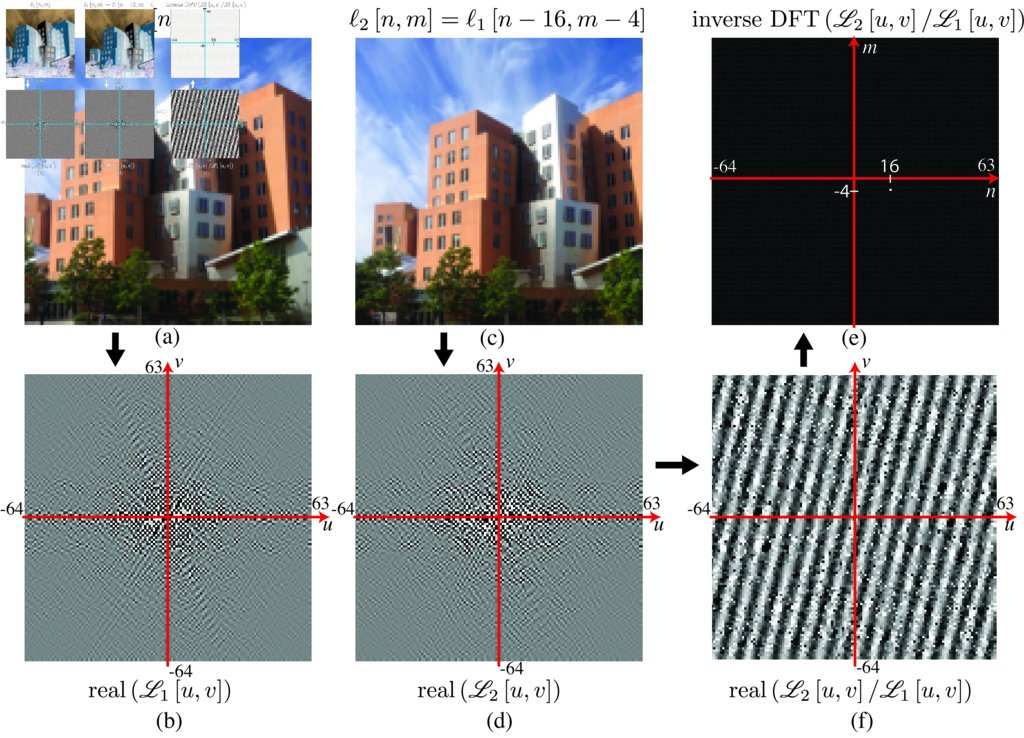
\includegraphics[width=1\linewidth]{figures/Image_processing_fourier/shiftFT2.eps}}
\caption{Translation in space. Image (c) corresponds to image (a) after a translation of 16 pixels to the right and four pixels down. Images (b) and (d) show the real parts of their corresponding DFTs (with $N=128$). Image (f) shows the real part of the ratio between the two DFTs, and (e) is the inverse transform of the ratio between DFTs. The inverse is very close to an impulse located at the coordinates of the displacement vector between the two images.} 
\label{fig:shiftFT}
\end{figure}

Locating the maximum on \fig{\ref{fig:shiftFT}}{f} can be used to estimate the displacement between two images when the translation corresponds to a global translation. However, this method is not very robust and it is rarely used in practice.


\subsection{Modulation, Translation in Frequency}

If we multiply an image with a complex exponential, its Fourier transform is translated, a property related to the previous one:

%\begin{equation}
%DFT \left\{ f\left[n,m \right]  \exp{ \left( -2\pi j \left( \frac{u_0\, n}{N} + \frac{v_0\, m}{M} \right) \right)} \right\}
%=
%F \left[u-u_0,v-v_0 \right]
%\end{equation}

\begin{equation}
\img \left[n,m \right]  \exp{ \left( -2\pi j \left( \frac{u_0\, n}{N} + \frac{v_0\, m}{M} \right) \right)}\xrightarrow{\mathscr{F}} 
\capitalimg \left[u-u_0,v-v_0 \right]
\label{eq:modulation_exp}
\end{equation}
This can be proven using the dual convolution property from section \sect{\ref{section:dualconv}}.
Note that now the result in \eqn{\ref{eq:modulation_exp}} is not a real signal, and for this reason its Fourier Transform does not have symmetries around $u,v=0$. 

A related relationship is as follows: 
%\begin{equation}
%DFT \left\{ f\left[n,m \right]  \cos{ \left( 2\pi j \left( \frac{u_0\, n}{N} + \frac{v_0\, m}{M} \right) \right)} \right\}
%=
%F \left[u-u_0,v-v_0 \right] + F \left[u+u_0,v+v_0 \right] 
%\end{equation}

\begin{equation}
\img \left[n,m \right]  \cos{ \left( 2\pi j \left( \frac{u_0\, n}{N} + \frac{v_0\, m}{M} \right) \right)}
\xrightarrow{\mathscr{F}} 
\capitalimg \left[u-u_0,v-v_0 \right] + \capitalimg \left[u+u_0,v+v_0 \right] 
\end{equation}

Multiplying a signal by a wave is called signal modulation and it is one of the basic operations in communications. It is also an important property in image analysis and we will see its use later. 

\Fig{\ref{fig:modulation}} shows an example of modulating an image of a stop sign by multiplying by diagonal wave. The bottom row shows the corresponding Fourier transforms.



\begin{figure}[t]
\centerline{
\includegraphics[width=1\linewidth]{figures/Image_processing_fourier/modulation.eps}}
\caption{Modulation in space. Multiplying an image by a cosine wave results in a new image with a Fourier transform with two copies of the Fourier transform of the original image. Only the magnitude of the Fourier transforms are shown.} 
\label{fig:modulation}
\end{figure}

Note that a shift and a modulation are equivalent operations in different domains. A shift in space is a modulation in the frequency domain and that a shift in frequency is a modulation in the spatial domain.


\section{A Family of Fourier Transforms}

The Fourier transform has a multitude of forms and it depends on the conventions used. When you will read papers or other books that make use of the Fourier transform, you will have to carefully check how are they defining the Fourier transform before using it in your own analysis. The important thing is to be consistent in the formulation. 

The Fourier transform also will change depending on the type of signal being analyzed. Although in this book we will mostly work with finite length discrete signals and images, it is worth defining the Fourier transform for other signals such as continuous signals (which are a function of a continuous independent variable such as time), or infinite length discrete signals for which the definition of the DFT will not be convenient. 


\subsection{Fourier Transform for Continuous Signals}

The continuous domain is convenient when working with functions and operations that are not defined in the discrete domain. For instance, the derivative operator is well defined in the continuous domain but we can only approximate it in the discrete domain. Another example is when using the Gaussian distribution, which is defined as a continuous function. For this reason, sometimes some formulation is easier when done in the continuous domain. 

For infinite length signals defined on the continuous domain, the Fourier transform is defined as:

\begin{equation}
\capitalimg (w) =  \int_{-\infty}^{\infty} \img (t) \exp{ \left( - j w t \right)} \, dt 
\label{eq:contfourier}
\end{equation}
where $\capitalimg (w)$ is a continuous function on the frequency $w$ (in radians). As before, this transform also has an inverse. The inverse Fourier transform is as follows:

\begin{equation}
\img (t) = \frac{1}{2 \pi} \int_{-\infty}^{\infty} \capitalimg (w) \exp{ \left( j w t \right) } \, dw
\label{eq:invcontfourier}
\end{equation}
Most of the properties that we have seen for the DFT also apply to the continuous domain, replacing sums with integrals. 

The convolution between two continuous signals is defined as
\begin{equation}
\imgout (t) =  \img_1 \circ \img_2 = \int_{-\infty}^{\infty} \img_1 (t-t') \img_2(t') \, d t' 
\label{eq:contconv}
\end{equation}
Those definitions can be extended to 2D dimensions by making all the integrals double and integrating across the spatial variables $x$ and $y$. Although, in practice, images and filters will be discrete signals, many times it is convenient to think of them as continuous signals.



\subsection{Fourier Transform for Infinite Length Discrete Signals}

Another useful tool is the Fourier transform for discrete signals with infinite length. In this case, the sum becomes infinite, and by replacing $w = 2 \pi u / N$ in \eqn{\ref{eq:fourier}}, we can write:
\begin{equation}
\capitalimg (w) = \sum_{n=-\infty}^{\infty} \img \left[n \right] \exp{(- j w n)}
\end{equation}
The frequency $w$ is now a continuous variable. The Fourier transform $\capitalimg (w)$ is a periodic function with period $2 \pi$. 

The inverse Fourier transform is
\begin{equation}
\img \left[n \right] = \frac{1}{2\pi} \int_{2 \pi} \capitalimg (w) \exp{(j w n)} d w
\end{equation}
where the integral is done only in one of the periods. 

Table \ref{table:tableFamilyFT} summarizes the three transforms we have seen in this chapter. All of them can be easily extended to 2D. There are more variations of the Fourier transform that we will not discuss here. 


\begin{table}[h]
%\marginnote{{\bf Table \ref{table:tableFamilyFT}}: Fourier transforms. There are many variants of the Fourier transform. Here we describe the ones we will use in this book.} % Hack to get the caption of the table in the margin.
\caption{Fourier transforms. There are many variants of the Fourier transform. Here we describe the ones we will use in this book.} % Hack to get the caption of the table in the margin.
%\faketablecaption{} % this updates the counter without plotting a caption.
%\caption{Fourier transforms}
\begin{center}
{
\renewcommand{\arraystretch}{2.5}
%\renewcommand{\tabcolsep}{0.2cm}
\begin{tabular}{| p{2.1cm} | c | c | p{2.1cm} |}
\hline
Time domain & FT & FT$^{-1}$ & Frequency domain \\
\hline \hline
Discrete time, Finite length ($N$) & 
$\displaystyle \capitalimg \left[u \right] = \sum_{n=0}^{N-1} \img \left[n \right] e^{-2 \pi j \frac{un}{N}}$
&
$\displaystyle \img \left[n \right] = \frac{1}{N} \sum_{u=0}^{N-1} \capitalimg \left[u \right] e^{2 \pi j \frac{un}{N} }$ &
Discrete frequency, Finite length ($N$) \\
\hline

Continuous time, Infinite length & 
$\displaystyle \capitalimg (w) = \int_{- \infty}^{\infty} \img (t) e^{- j w t} dt$
&
$\displaystyle \img (t) = \frac{1}{2\pi} \int_{- \infty}^{\infty} \capitalimg (w) e^{j w t} d w$ &
Continuous frequency, Infinite length \\
\hline

Discrete time, Infinite length & 
$\displaystyle \capitalimg (w) = \sum_{n=-\infty}^{\infty} \img \left[n \right] e^{- j w n}$
&
$\displaystyle \img \left[n \right] = \frac{1}{2\pi} \int_{2 \pi} \capitalimg (w) e^{j w n} d w$ &
Continuous frequency, Finite length ($2 \pi$) \\
\hline
\end{tabular}
}
\end{center}
\label{table:tableFamilyFT} 
\end{table}


\section{Fourier Analysis as an Image Representation}

The Fourier transform has been extensively used as an image representation. In this section we will discuss the information about the picture that is made explicit by this representation.


As we discussed before, the Fourier transform of an image can be written in polar form:
\begin{equation}
\capitalimg \left[u,v \right]  = A \left[u,v \right] \, \exp{\left( j\, \theta\left[u,v \right]  \right)}
\end{equation}
where $A \left[u,v \right] = \left| \capitalimg \left[u,v \right]  \right|$ and $\theta \left[u,v \right] = \angle  \capitalimg \left[u,v \right]$.

 
\marginnote{Decomposing the Fourier transform of a signal in its amplitude and phase can be very useful. It has been a popular image representation during the early days of computer vision and image processing.}[-.5in]
If we think in terms of the inverse of the Fourier transform, $A \left[u,v \right]$ gives the strength of the weight for each complex exponential and the phase $\theta \left[u,v \right]$ translates the complex exponential. The phase carries the information of where the image
contours are by specifying how the phases of the sinusoids must line up in order to create the observed contours and edges. In fact, as shown in section~\ref{section:DFTproperties}, translating the image in space only modifies the phase of its Fourier transform. In short, one can think that location information goes into the phase while intensity scaling goes into the magnitude. 

One might ask which is more important in determining the appearance of the image, the magnitude
of the Fourier transform, or its phase.  \Fig{\ref{fig:phaseoramp}} shows the result of a classical experiment that consists of computing the Fourier transform for two images and building two new images by swapping their phases \cite{Oppenheim1981}. 


\begin{figure}
\centerline{
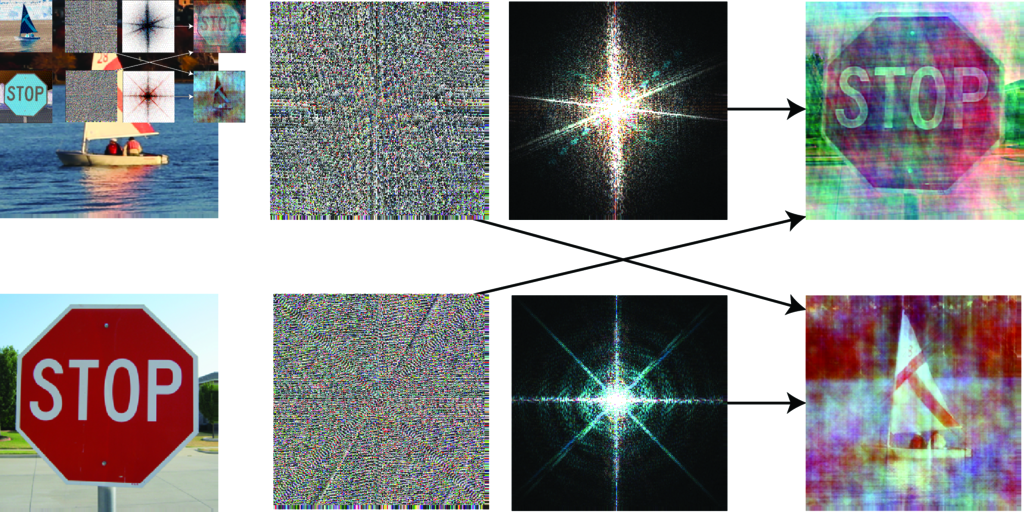
\includegraphics[width=1\linewidth]{figures/Image_processing_fourier/amp_phase_swap_color.eps}}
\caption{Swapping the amplitude and the phase of the Fourier Transform of two images. Each color channel is processed in the same way.}
\label{fig:phaseoramp}
\end{figure}

The first output image is the inverse Fourier transform of the amplitude of the first input image and the phase of the DFT of the second input image. The second output image contains the other two terms. The figure shows that the appearance of the resulting images is mostly dominated by the phase of the image they come from. The image built with the phase of the stop sign looks like the stop sign even if the amplitude comes from a different image. \Fig{\ref{fig:phaseoramp}} shows the result in color by doing the same operation over each color channel (red, green, and blue) independently. The phase signal determines where the edges and colors are located in the resulting image. The final colors are altered as the amplitudes have changed. 


\marginnote{A remarkable property of natural images: the magnitude of their DFT generally has its maximum at the origin and decays inversely proportional to the radial frequency.}[0in]
One remarkable property of real images is that the magnitude of the DFT of natural images is quite similar and can be approximated by $A \left[u,v \right] = a/ (u^2+v^2)^b$ with $a$ and $b$ being two constants. We will talk more about this property when discussing statistical models of natural images in \chap{\ref{chapter:stat_image_models}}. This typical structure of the DFT magnitude of natural images has been used as a prior for many tasks such as image denoising.


\begin{figure}[t]
\centerline{
\includegraphics[width=1\linewidth]{figures/Image_processing_fourier/dft_random_phaseandamplitude.eps}}
\caption{The relative importance of phase and amplitude depends on the image. Each row shows one image, its Fourier transform (amplitude and phase), and the resulting images obtained by applying the inverse Fourier transform to a signal with the original amplitude and randomized phase, and a signal with the original phase and a generic fixed $1/f$ amplitude. Note that for the first image, the phase seems to be the most important component. 
%However, as we move down, the relative importance between the two components changes. And for the bottom image (showing a pseudo-periodic threat texture) the amplitude is the most important component.
}
\label{fig:phasevsamp}
\end{figure}

However, this does not mean that all the information of the image is contained inside the phase only. The amplitude contains very useful information as shown in \fig{\ref{fig:phasevsamp}}. To get an intuition of the information available on the amplitude and phase let's do the following experiment: let's take an image, compute the Fourier transform, and create two images by applying the inverse Fourier transform when removing one of the components while keeping the other original component. For the amplitude image, we will randomize the phase. For the phase image, we will replace the amplitude by a noninformative $A \left[u,v \right] = 1/(u^2+v^2)^{1/2}$ for all images. This amplitude is better than a random amplitude because a random amplitude produces a very noisy image hiding the information available, while this generic form for the amplitude will produce a smoother image, revealing its structure while still removing any information available on the original amplitude. \Fig{\ref{fig:phasevsamp}} shows different types of images and how the DFT amplitude and phase contribute to defining the image content. The top image is inline with the observation from \fig{\ref{fig:phaseoramp}} where phase seems to be carrying most of the image information. However, the rest of the images do not show the same pattern. As we move down along the examples in the figure, the relative importance between the two components changes. And for the bottom image (showing a pseudo-periodic thread texture) the amplitude is the most important component.


The amplitude is great for capturing images that contain strong periodic patterns. In such cases, the amplitude can be better than the phase. This observation has been the basis for many image descriptors \cite{Gorkani94,oliva01}. The amplitude is somewhat invariant to location (although it is not invariant to the relative location between different elements in the scene). However the phase is a complex signal that does not seem to make explicit any information about the image.

%Exercise: reproduce the figure \ref{fig:phasevsamp} but in color. For this to work, it is better to do PCA in color space first to rotate the color space to three channels that are decorrelated, then build each decorrelated channel independently and then merge undoing the rotation to get an RGB image. In the color chapter we will see better examples of why this rotation is important. 

%\subsection{Orientations and scales}
%
%(needs to be written)
%
%Another way in which the Fourier transform is useful is because it makes explicit which components contribute to different scales and different orientations. 
%
%Show some examples to illustrate how to read orientation and scale.
%
%FIGURE: rocks of different sizes. textures of different orientations.



%\subsection{Images in the Fourier domain}
%
%(needs to be written)
%
%- show pictures in which basic frequencies are visible: waves in the water, images with strong periodic patterns and show their fourier transforms
%
%- table of some basic images and their 2D fourier transforms (e.g, a wave, a rectangle, a circle, an oriented line, a segment, a dot, ...)
%
%- discuss the issue about visualizing the power spectrum of natural images to avoid DC component. Also, use a window to avoid the vertical and horizontal lines in the power spectrum due to the boundary artifacts.
%
%- game A B C, 1 2 3: maybe make it add a few more examples to make it more challenging and interesting. 
%
%
%
%%IDEA: can we extract the pattern that gets repeated?
%
%

\begin{figure}[H]
\centerline{
\includegraphics[width=1.0\linewidth]{figures/Image_processing_fourier/FTgame.eps}}
\caption{The Fourier transform matching game: Match each image (a-h) with its corresponding Fourier transform magnitude (1-8).}
\label{fig:quiz}
\end{figure}


Take the following quiz: match the Fourier transform magnitudes with the corresponding images in \fig{\ref{fig:quiz}}\footnote{The correct answers to the quiz \fig{\ref{fig:quiz}} are 1-h, 2-f, 3-g, 4-c, 5-b, 6-e, 7-d, and 8-a.}. Some image patterns are easily visible in the Fourier domain. For instance, strong image contrasts produce oriented lines in the Fourier domain. Periodic patterns are also clearly visible in the Fourier domain. A periodic pattern in the image domain produces periodic impulses in the Fourier domain. The location of the impulses will be related to the period and orientation or the repetitions. 






\section{Fourier Analysis of Linear Filters}
\label{sect:transfer_function}

Linear convolutions, despite their simplicity, are surprisingly useful for processing and interpreting images.  
It's often very useful to blur images, in preparation for subsampling or to remove noise, for example.  Other useful processing includes
edge enhancement and motion analysis. From the previous section we know that we can write linear filters as convolutions:
%\begin{equation}
%y \left[n,m \right] = h \left[n,m \right] \circ x \left[n,m \right]
%\label{eq:lin}
%\end{equation}
\begin{center}
\tikzstyle{int}=[draw, minimum size=3em]
\tikzstyle{init} = [pin edge={to-,thin,black}]
\begin{tikzpicture}[node distance=0cm,auto,>=latex']
  \node [int] (box1) {$h \left[ n,m \right]$};
   \node [left of=box1,node distance=2.0cm] (input) {$\imgin \left[ n,m \right]$};
   \node [right of=box1,node distance=3.5cm] (output) {$\imgout \left[ n,m \right] = h \left[n,m \right] \circ \imgin \left[n,m \right]$};
    \node (c) [right of=box1,node distance=3cm, coordinate] {};
    \path[->] (input) edge node {} (box1);
    \path[->] (box1) edge node {} (output);
\end{tikzpicture}
\end{center}
where $h \left[n,m \right]$ is the impulse response of the system, or convolution kernel.
We can also write this as a product in the Fourier domain:
%\begin{equation}
%Y \left[u,v \right] = H \left[u, v \right] X \left[u, v \right]
%\label{eq:dft-lin}
%\end{equation}


%\begin{figure}[h!]
\begin{center}
\tikzstyle{int}=[draw, minimum size=3em]
\tikzstyle{init} = [pin edge={to-,thin,black}]
\begin{tikzpicture}[node distance=0cm,auto,>=latex']
  \node [int] (box1) {$H \left[ u,v \right]$};
   \node [left of=box1,node distance=2.0cm] (input) {$\capitalimgin \left[ u,v \right]$};
   \node [right of=box1,node distance=3.5cm] (output) {$\capitalimgout \left[ u,v \right] = H \left[u, v \right] \capitalimgin \left[u, v \right]$};
    \node (c) [right of=box1,node distance=3cm, coordinate] {};
    \path[->] (input) edge node {} (box1);
    \path[->] (box1) edge node {} (output);
\end{tikzpicture}
\end{center}
%\label{fig:genericfilterH}
%\end{figure}
The function $H \left[u, v \right]$ is called the {\bf transfer function} of the filter. 
\marginnote{The transfer function of a filter is the Fourier transform of the convolution kernel.}
The transfer function will allow us interpret filters by how they modify the spectral content of the input signal. As the Fourier transform of the output is just a product between the Fourier transform of the input and the transfer function, a linear filter simply reweights the spectral content of the signal. It does not create new content, it can only enhance or decrease the spectral components already present in the input. \marginnote{A convolution between two signals does not create new spectral content. To create new spectral components not present in the input we need to apply nonlinearities.}

If we use the polar form:
\begin{equation}
H \left[u,v \right] = \left|H \left[u, v \right] \right| \exp \left( {j \, \angle H \left[u, v \right]} \right)
\label{eq:polar-lin}
\end{equation}
The magnitude $\left| H \left[u, v \right] \right|$ is the {\bf amplitude gain}, and the phase $\angle H \left[u, v \right] $ is the {\bf phase shift}. The magnitude at the origin, $\left| H \left[0, 0 \right] \right|$, is the {\bf DC gain} of the filter (the average value of the output signal is equal to the average value of the input times the DC gain). 
\index{DC gain}

The Fourier domain shows that, in many cases, what a filter does is to block or let pass certain frequencies. Filters are many times classified according to the frequencies that they let pass through the filter (low, medium, or high frequencies) as shown in \fig{\ref{fig:typestypes}}.

\begin{figure}[H]
\centerline{
\includegraphics[width=.9\linewidth]{figures/Image_processing_fourier/filter-types.eps}
}
\caption{Sketch of the frequency responses of low-pass, band-pass, and high-pass filters.}
\label{fig:typestypes}
\end{figure}

%\begin{itemize}
%\item Low-pass filter
%\item Band-pass filter
%\item High-pass filter
%\end{itemize}

When filtering images, low-pass filters will output a blurry picture encoding the {\bf coarse} elements of the image. A band-pass filter will highlight middle size elements, while the output of a high-pass filter will show the {\bf fine} details of the image. The three images in \fig{\ref{fig:sketchresponses}} show the output image processed by three filters corresponding to the frequency responses of \fig{\ref{fig:typestypes}}.

\begin{figure}[h]
\centerline{

\includegraphics[width=.3\linewidth]{figures/linear_image_filtering/sketch_coarse.jpg}
~
\includegraphics[width=.3\linewidth]{figures/linear_image_filtering/sketch_middle.jpg}
~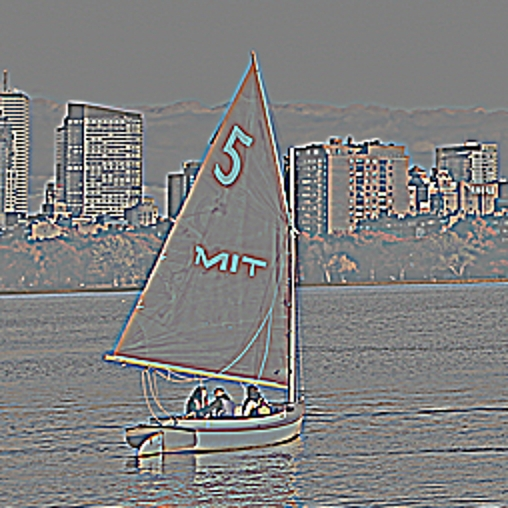
\includegraphics[width=.3\linewidth]{figures/linear_image_filtering/sketch_fine.jpg}
}
\caption{An image filtered by (left) low-pass, (middle) band-pass, and (right) high-pass filters.}
\label{fig:sketchresponses}
\end{figure}


There are many other properties of a filter that can be used to classify linear systems (e.g., causality, stability, phase-changes). Some filters have their main effect over the phase of the signal and they are better understood in the spatial domain. In general, filters affect both the magnitude and the phase of the input signal.

%
%
%Michelson contrast:
%\begin{equation}
%(Imax-Imin)/(Imax+Imin)  
%\end{equation}
%
%Weber contrast:  $\Delta I / I$.
%




Let's now look at two examples of the application of the Fourier analysis of linear filters.  


\subsection{Example 1: Removing the Columns from the MIT Building}

\Fig{\ref{fig:filteringFT}}{a} shows a picture of the main MIT building. The columns produce a quasiperiodic pattern. \Fig{\ref{fig:filteringFT}}{b} shows the magnitude of the DFT of the MIT picture. One can see picks in the horizontal frequency axis, those picks are due to the columns. 

To check this we can verify first that the location of the picks is related to the separation of the columns. The image in \fig{\ref{fig:filteringFT}}{a} has a size of $256\times256$ pixels, and the columns are repeated every 14 pixels. Therefore, the DFT, with $N=256$, will have picks at the horizontal frequencies: $256/14=18.2$, which is indeed what we observe in \fig{\ref{fig:filteringFT}}{b}. As the repeated pattern is not a pure sinusoidal function, there will be picks at all the harmonic frequencies $k\frac{256}{14}$, where $k$ is an integer. Note also that the picks seem to produce vertical bands with decreasing amplitude with increasing vertical frequency $v$. These bands occur because the columns only occupy a small vertical segment of the image. Also, as the columns only exist in a portion of the horizontal region of the image, the picks also have some horizontal width. 

We can now also check the effect of suppressing those frequencies by zeroing the magnitude of the DFT around each pick (here we zero 7 pixels in the horizontal dimension and all the pixels along the vertical dimension) as shown \fig{\ref{fig:filteringFT}}{d}. \Fig{\ref{fig:filteringFT}}{c} shows the resulting image where the columns are almost gone while the rest of the image is little affected. \Fig{\ref{fig:filteringFT}}{e} shows the complementary image (in fact, $a=c+e$) and its DFT in \fig{\ref{fig:filteringFT}}{f}.

\begin{figure}[t]
\centerline{
\includegraphics[width=1\linewidth]{figures/Image_processing_fourier/mit_columns.eps}}
\caption{Simple filtering in the Fourier domain.  (a) The repeated columns of the
  building of the MIT dome generate harmonics along a horizontal line
  in the Fourier domain shown in (b). By zeroing out those Fourier
  components, as done in (d), the columns of the building are substantially removed (c). We can also the complementary operation keeping only those harmonics, shown in (f), which results in keeping only the columns (e).
} 
\label{fig:filteringFT}
\end{figure}


\subsection{Example 2: The Human Visual System and the Contrast Sensitivity Function}

Before we start describing different types of linear filters in the next chapters, let's start by gaining some subjective experience by playing with one: our own visual system. Although our visual system is clearly a nonlinear system, linear filter theory can explain some aspects of our perception. Indeed, under certain conditions, the first stages of visual computation perform of the visual system can be approximated by a linear filter. 

Fourier analysis and the use of sine waves became very popular in the field of visual psychophysics. {\bf Visual psychophysics}
\index{Visual psychophysics}
is an experimental science that studies the relationship between real world stimuli and our perception.
\marginnote{The concept of {\bf psychophysics} was introduced by Gustav Theodor Fechner (1801--1887).
\\[6pt]
\centerline{
\setlength{\fboxsep}{0pt}
\fbox{

\includegraphics[width=.4\linewidth]{figures/Image_processing_fourier/experimental_setup.jpg}
}
}
}[-1.3in]

Using the theory we have studied in this chapter, we can show that when the input to a linear system is a wave of frequency $u_0$ and amplitude 1, the output is another wave of the same frequency as the input but with an amplitude equal to $|H \left[ u_0 \right]|$: 

%\begin{figure}[h!]
\begin{center}
\tikzstyle{int}=[draw, minimum size=3em]
\tikzstyle{init} = [pin edge={to-,thin,black}]
\begin{tikzpicture}[node distance=0cm,auto,>=latex']
  \node [int] (box1) {$H \left[ u \right]$};
   \node [left of=box1,node distance=2.0cm] (input) {$\exp \left(2 \pi j   \frac{u_0\, n}{N}   \right)$};
   \node [right of=box1,node distance=3.25cm] (output) {$|H \left[ u_0 \right]| \exp \left(2 \pi j   \frac{u_0\, n}{N} + j \angle H \left[ u \right]   \right)$};
    \node (c) [right of=box1,node distance=3cm, coordinate] {};
    \path[->] (input) edge node {} (box1);
    \path[->] (box1) edge node {} (output);
\end{tikzpicture}
\end{center}
%\label{fig:genericfilterH}
%\end{figure}

This means that one way of identifying the transfer function of a system is by using as input a wave and measuring the output amplitude as a function of the input frequency $u_0$. This inspired a generation of psychophysicists to study how the human visual system behaved when presented with periodic signals. 


To experience the transfer function of our own visual system, let's build the following $N \times M$ image:
\begin{equation}
\img \left[n,m\right] = A\left[m\right] \sin(2 \pi f\left[n\right] n/N)
\end{equation}
with
\begin{equation}
A\left[m\right] = A_{min} \left(\frac{A_{max}}{A_{min}}\right)^{m/M}
\end{equation}
and
\begin{equation}
f\left[n\right] = f_{min} \left(\frac{f_{max}}{f_{min}}\right)^{n/N}
\end{equation}
This image is separable and it is composed of two factors: an amplitude, $A\left[m\right]$, that varies only along the vertical dimension, $m$, and a wave with a frequency, $f\left[n\right]$, that varies along the horizontal component, $n$. The amplitude, $A\left[m\right]$, goes from $A_{max}$ to $A_{min}$ on a logarithmic scale. The frequency function, $f\left[n\right]$, is defined as an increasing function that starts from $f_{min}=1$ and grows up to $f_{max}=60$ (with $N=2,048$ being the number of horizontal pixels in the image). This image is shown in \fig{\ref{fig:csfchart}} and it is also called the {\bf Campbell and Robson chart}.
\index{Campbell and Robson chart}
It appears to an observer as a signal with a wave that oscillates slow at the left and faster toward the right and that has high contrast a the bottom and loses contrast towards the top becoming invisible.


\begin{figure}[t]
\centerline{
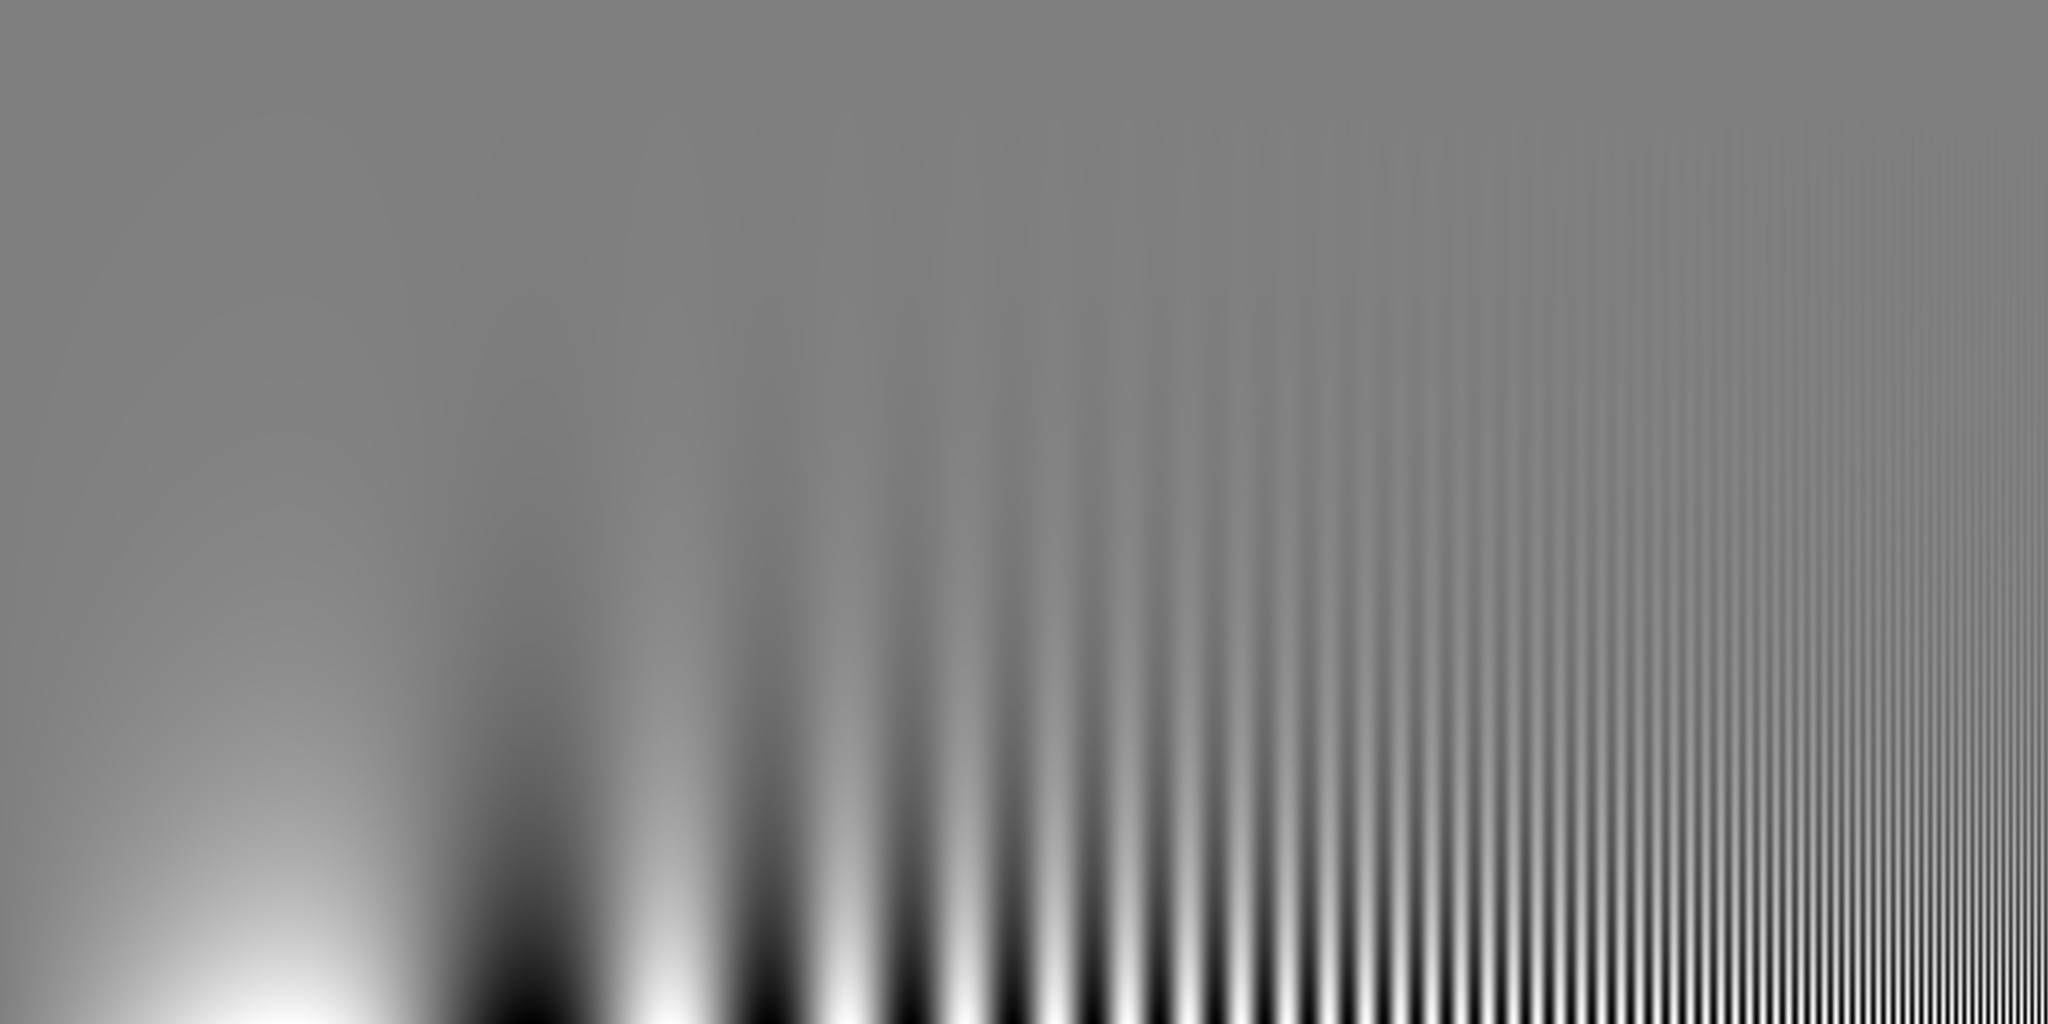
\includegraphics[width=1\linewidth]{figures/spatial_filters/csf.jpg}
} 
\caption{Contrast sensitivity function shown by the Campbell and Robson chart. The image shows a sine wave of increasing frequency from left to right, and increasing amplitude from top to bottom. Can you trace a curve over the chart to indicate where the sine wave becomes invisible?} 
\label{fig:csfchart}
\end{figure}


The first sign that our visual system is nonlinear is that we do not perceive the amplitude as changing exponentially fast from top to bottom. It feels more linear. This is because our photo-receptors compute the $\log$ of the incoming intensity (approximately).

What is interesting is that \fig{\ref{fig:csfchart}} is not perceived as being separable. If you trace the region where the sine wave seems to disappears you will trace a curve. 
%In fact, your visual system is behaving as a band-pass filter: you are sensitive to middle spatial frequencies (with a pick around 6 cycles/degree) and you are less sensitive for very low spatial frequencies (left of the image) and to high-spatial frequencies (right of the image). 
In fact, your visual system acts like a band-pass filter: you are sensitive to middle spatial frequencies (peaking around 6 cycles/degree) and less sensitive to very low spatial frequencies (on the left of the image) and high spatial frequencies (on the right of the image).
%This curve is called the contrast sensitivity function (CSF) in the psychophysics literature and is closely related to the transfer function of the filter, $H \left[ u,v \right]$, that  approximates our visual system. 
This curve, known as the contrast sensitivity function (CSF)
\index{Contrast sensitivity function}
in psychophysics literature, closely resembles the magnitude of the transfer function of the filter, $H \left[ u,v \right]$, which approximates the human visual system \cite{de1988spatial}.


The CSF is not a simple linear function but it can be approximated by one under certain conditions. However, the CSF changes depending of many factors such as overall intensity (the pick moves toward the left under low illumination.), adaptation (long exposure to one frequency reduces the sensitivity for that frequency), age, and so on. 

\marginnote{Here is my own CSF, traced by hand, with and without eyeglasses. Can you guess which one is with eyeglasses? 
\\[6pt]
\centerline{
\includegraphics[width=.5\linewidth]{figures/spatial_filters/my_CST.eps}
}
\\[6pt]
(Answer: the red curve is my CSF wearing eyeglasses.)
}[-1.5in]


\section{Concluding Remarks}

The Fourier transform is an indispensable tool for linear systems analysis,
image analysis, and for efficient filter output computation.  
Among the benefits of the Fourier transform representation are that it's easy
to analyze images according to spatial frequency, and this represents some progress in interpreting the image over merely a pixel representation.  But the Fourier transform has a major drawback
as an image representation: it's too global!  Every sinusoidal
component covers the entire image.  The Fourier transform tells us a
little about {\bf what} is happening in the image (based on the spatial
frequency content), but it tells us nothing about {\bf where} it is happening.  

Conversely, a pixel representation gives great spatial localization, but a pixel value by itself doesn't help us learn much about what's going on in the image.  A Fourier representation tells us a bit about what's going on, but nothing about where it happens.  We seek a representation that's somewhere in between those two extremes.

In the next chapters we will analyze several important linear filters. We will study spatial filters first, and then temporal filters. The filters we will study provide a foundation to understand many basic image processing operations, and to interpret learned filters by neural networks.

